\chapter{Instalacja i pierwsze uruchomienie -- instrukcja krok po kroku}
\label{cha:instalacjaIPierwszeUruchomienie}


Aplikacja \textit{HowAreYou} nie zostanie zainstalowana w klasyczny sposób. Zamiast sklepu Play do instalacji zostanie wykorzystana przeglądarka. Użytkownik musi przejść poprzez 3 etapy, które pozwolą na poprawdą instalację, konfigurację i uruchomienie aplikacji klienta oraz pluginu \textit{HowAreYou}.

%---------------------------------------------------------------------------

\section{Etap 1: Zezwolenie na instalację dodatkowych pakietów}
\label{sec:zezwolenieNaInstalacjeDodatkowychPakietow}

W pierwszej kolejności pozwolimy przeglądarce na instalację dodatkowych pakietów.

\begin{enumerate}
	
	\item Przejdź do \textit{Ustawień} systemu Android.
	
	\item Wybierz \textit{Aplikacje i powiadomienia}, a następnie \textit{Zaawansowane}.
	
	\begin{figure}[H]
		\centering
		\begin{subfigure}{0.35\textwidth}
			\centering
			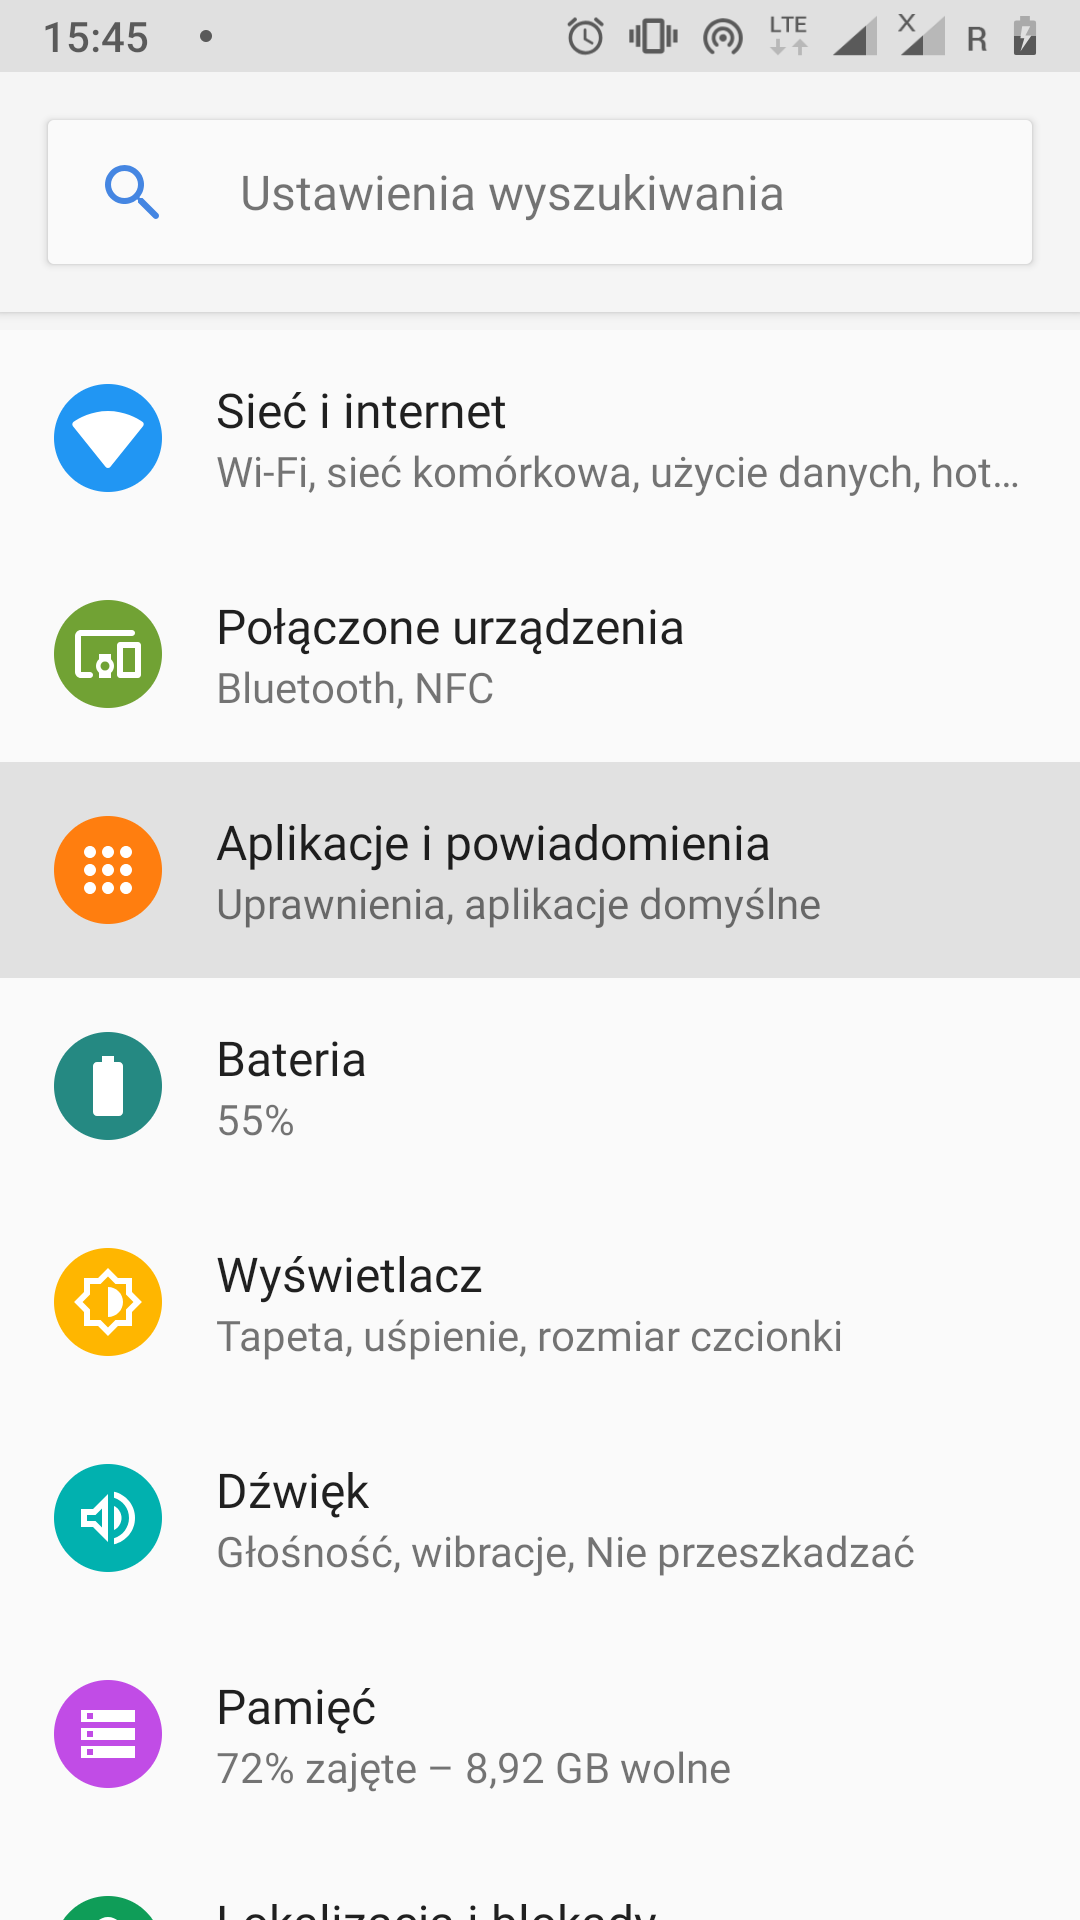
\includegraphics[scale=0.14]{dodatekA/1_1.png}
			\subcaption{\label{subfigure_a}}
		\end{subfigure}
		\begin{subfigure}{0.35\textwidth}
			\centering
			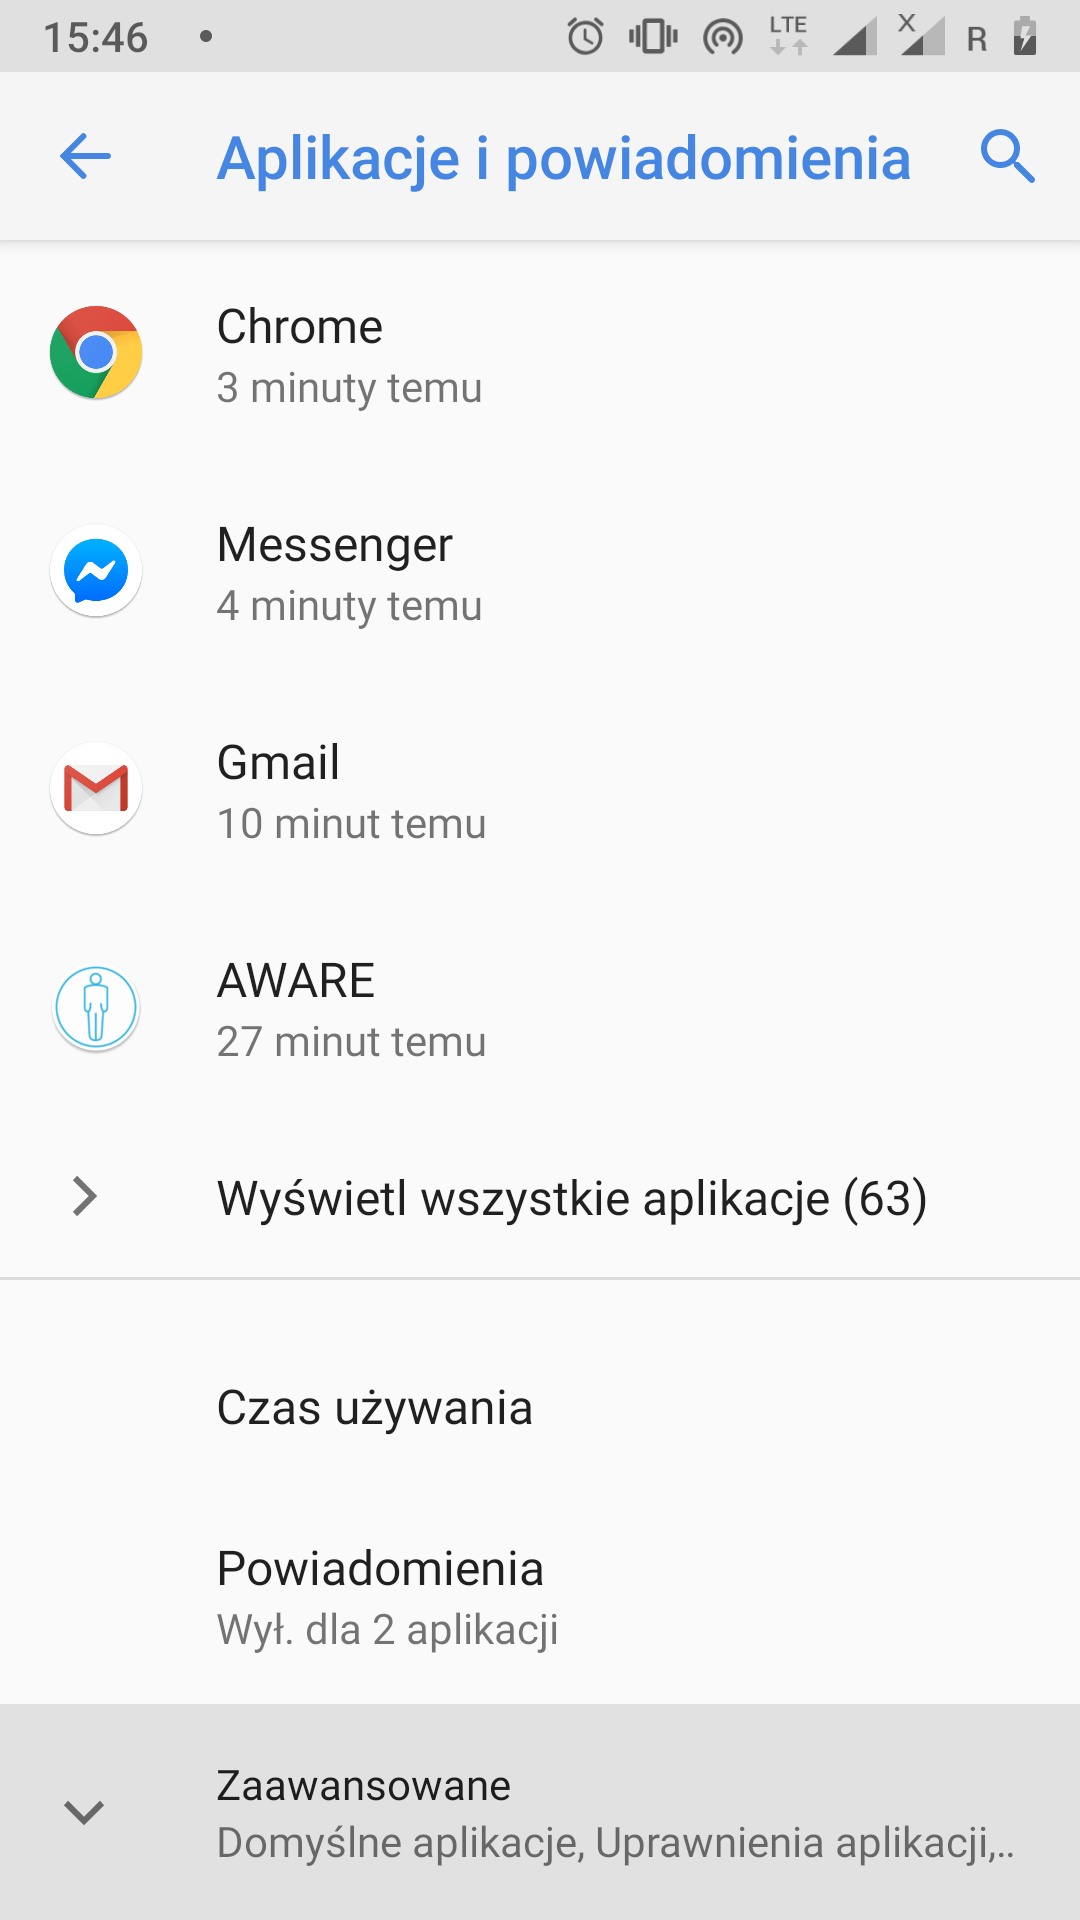
\includegraphics[scale=0.14]{dodatekA/1_2.png}
			\subcaption{\label{subfigure_b}}
		\end{subfigure}
		\caption{ Kroki 1 i 2: Przejście do zaawansowanych ustawień aplikacji.}
	\end{figure}
	
	\item Wybierz \textit{Specjalny dostęp do aplikacji}, a następnie \textit{Instalowanie nieznanych aplikacji}.
	
	\item Znajdź przeglądarkę, którą na co dzień używasz.
	
	\begin{figure}[H]
		\centering
		\begin{subfigure}{0.35\textwidth}
			\centering
			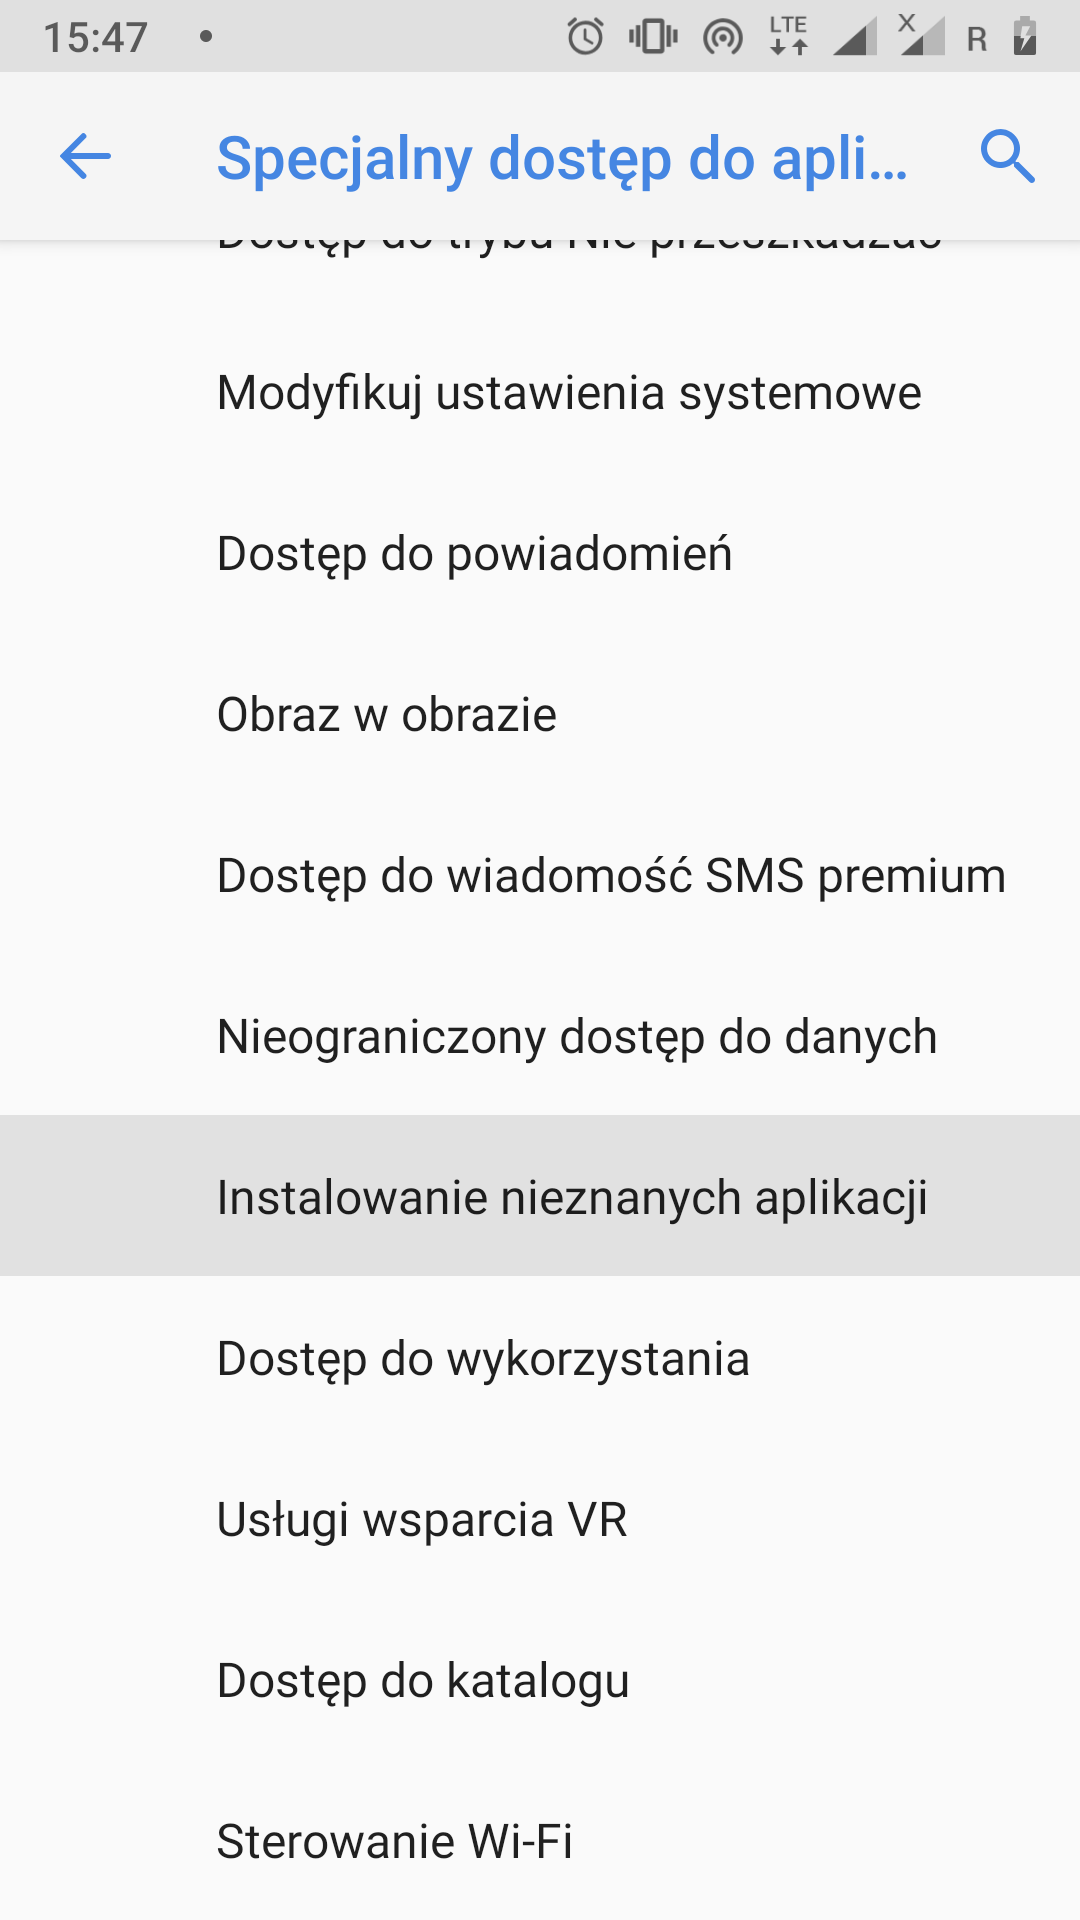
\includegraphics[scale=0.14]{dodatekA/1_3.png}
			\subcaption{\label{subfigure_a}}
		\end{subfigure}
		\begin{subfigure}{0.35\textwidth}
			\centering
			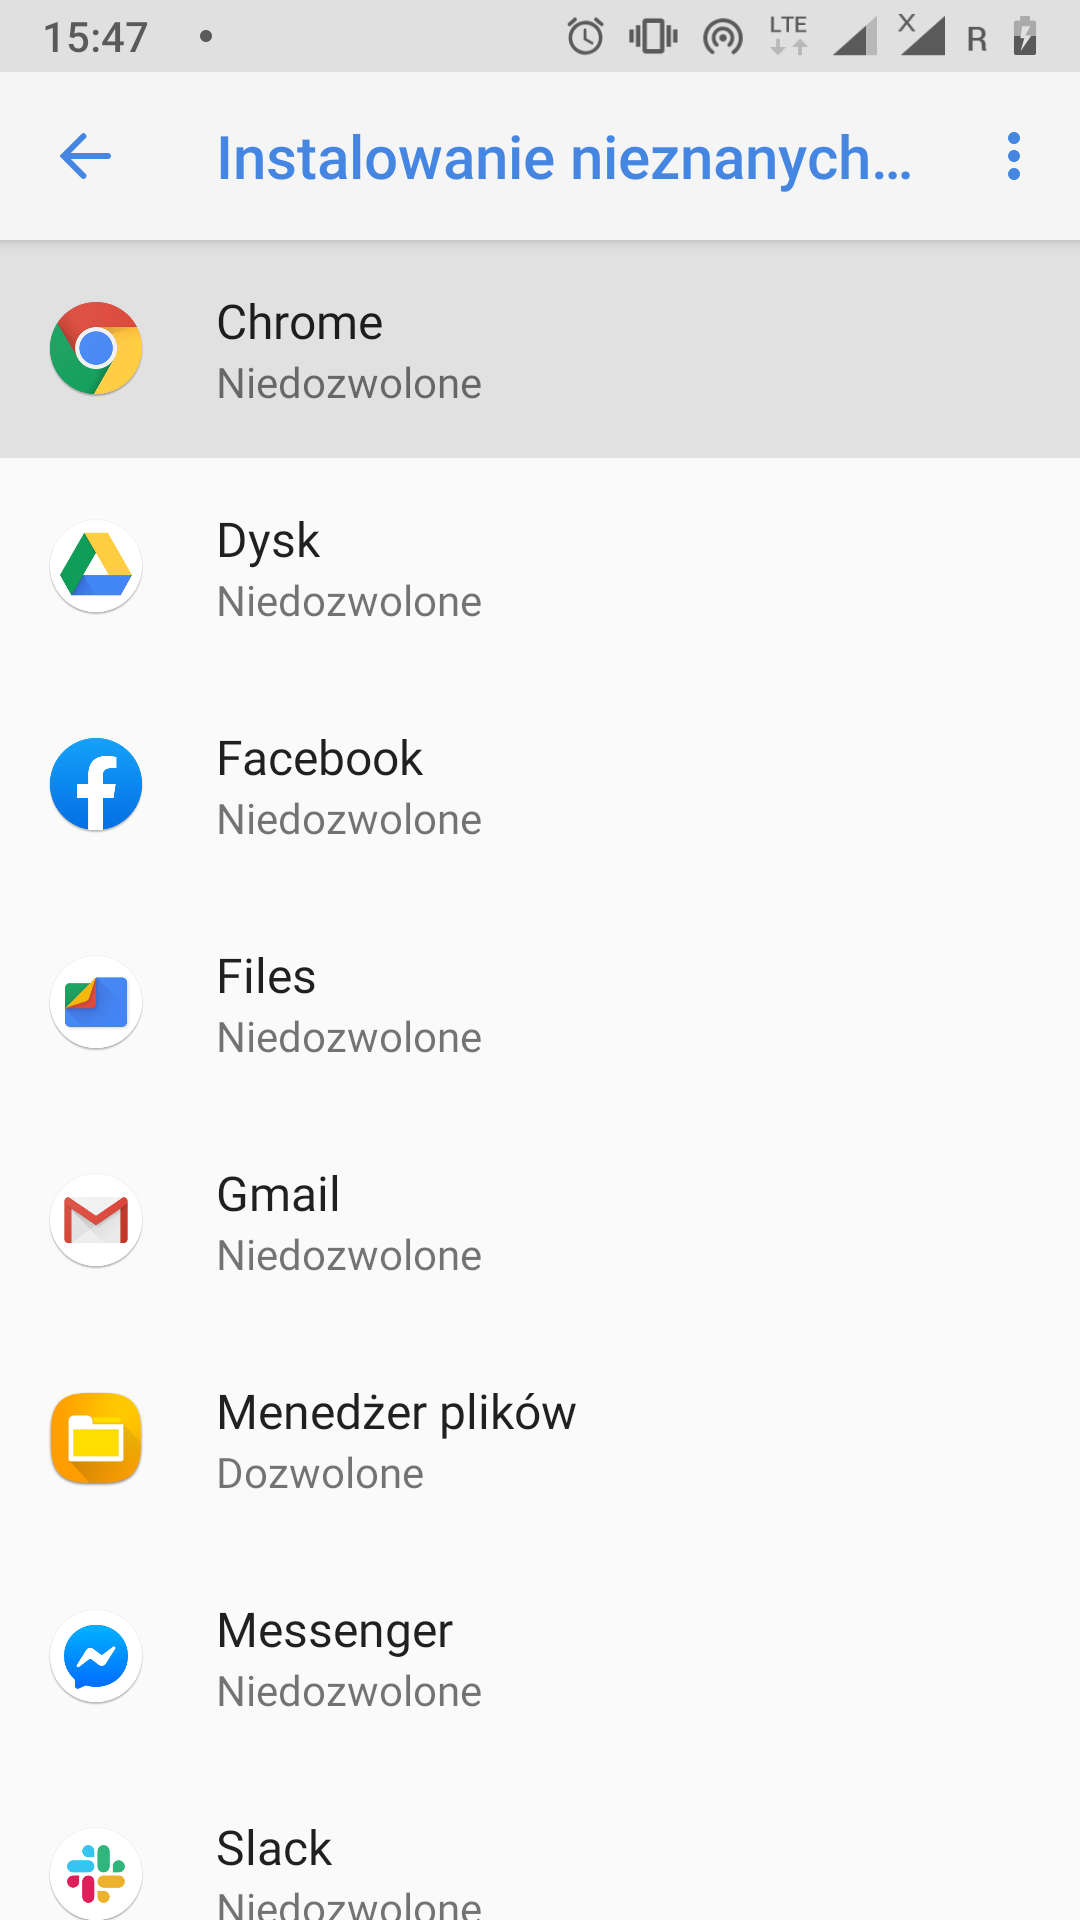
\includegraphics[scale=0.14]{dodatekA/1_4.png}
			\subcaption{\label{subfigure_b}}
		\end{subfigure}
		\caption{ Kroki 3 i 4: Aktywność \textit{Specjalny dostęp do aplikacji} (a) oraz aktywność \textit{Instalowanie nieznanych aplikacji} (b).}
	\end{figure}
	\clearpage 
	
	\item Kliknij \textit{Zezwól z tego źródła}.
	
	\begin{figure}[H]
		\centering
		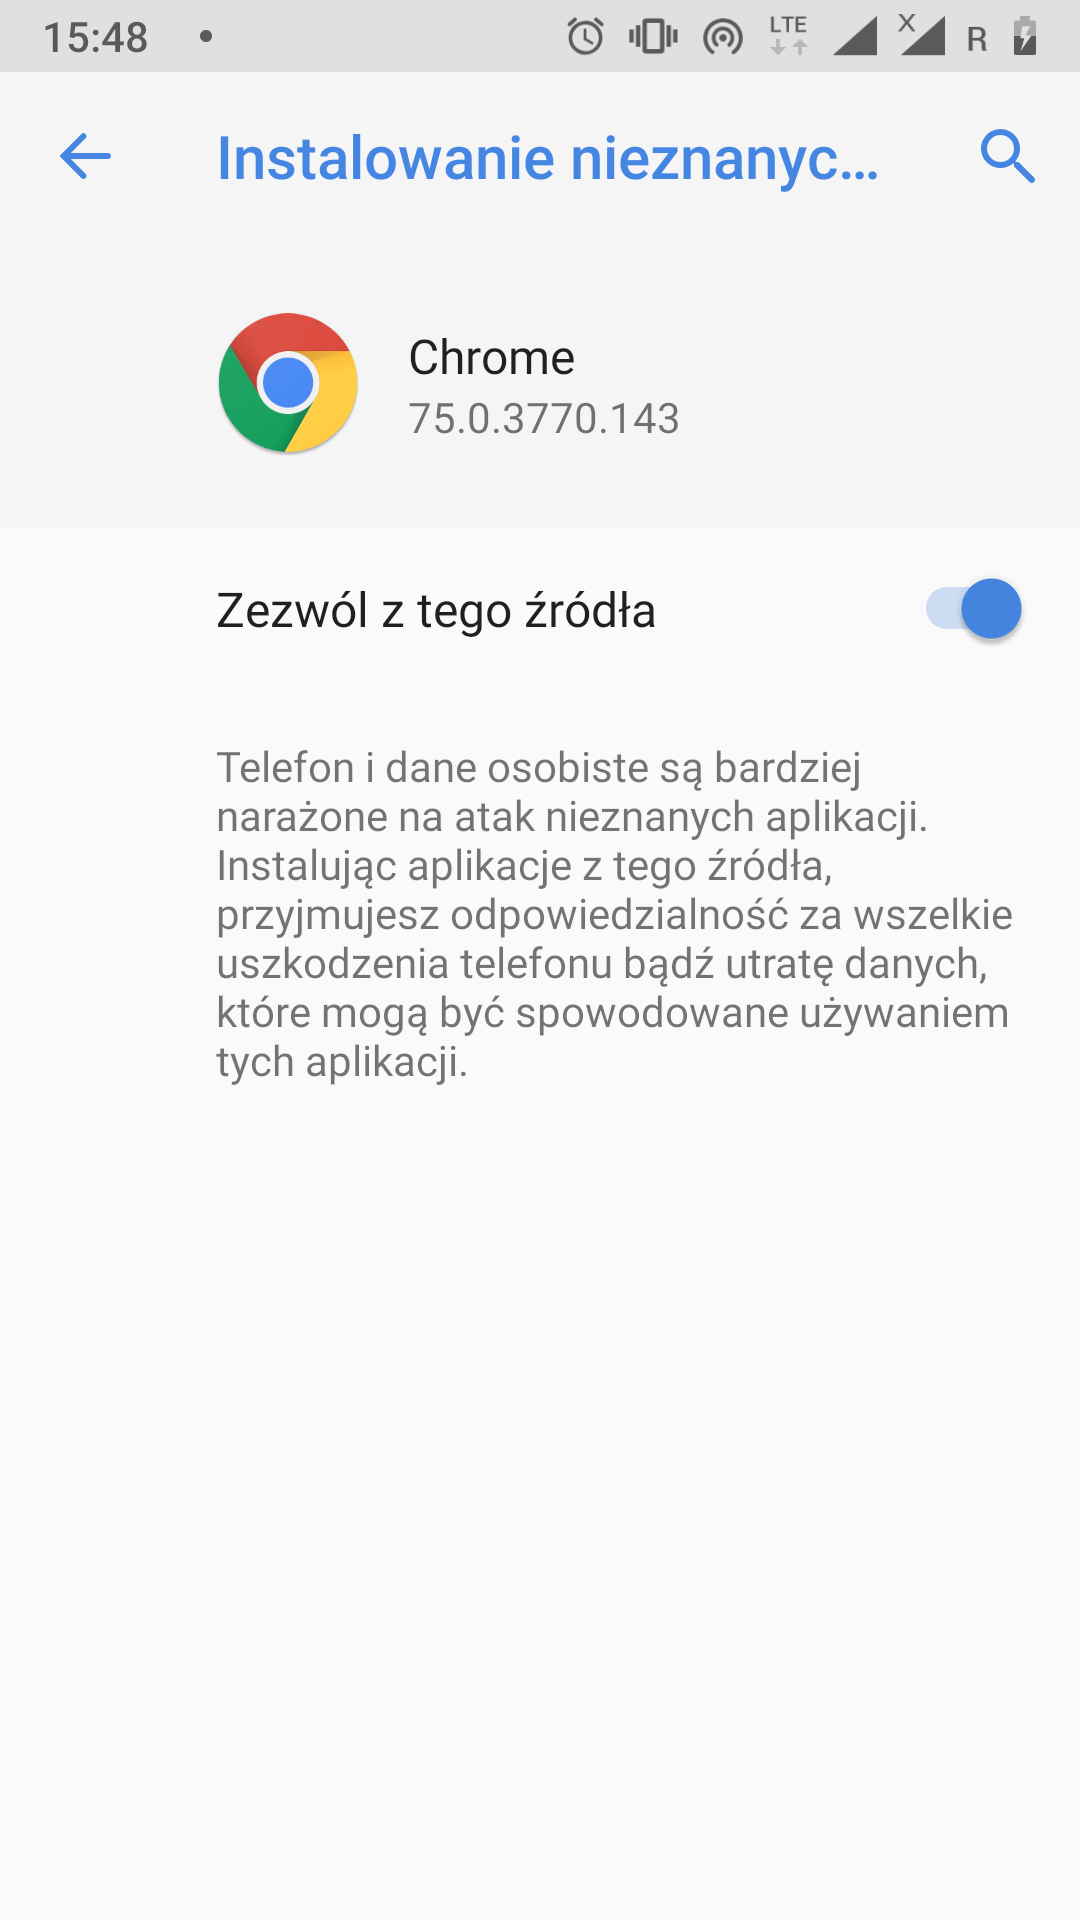
\includegraphics[scale=0.14]{dodatekA/1_5.png}
		\caption{Krok 5: Aktywność ustawień aplikacji.}
	\end{figure}
	
\end{enumerate}
\clearpage 

%---------------------------------------------------------------------------

\section{Etap 2: Pobranie i instalacja aplikacji}
\label{sec:pobranieIInstalacjaAplikacji}

Następnie pobierzemy i zainstalujemy aplikacje potrzebne do przeprowadzenia badania.

\begin{enumerate}
	
	\item W przeglądarce telefonu, którą wybrałeś w poprzednim kroku, odwiedź stronę \url{tiny.cc/97tz9y} lub \url{https://github.com/filipbiernat/HowAreYou_plugin/wiki/Linki-do-instalacji-HowAreYou}.
	
	\item Pobierz plik instalatora klikając na \textit{AwareClient}.
	
	\begin{figure}[H]
		\centering
		\begin{subfigure}{0.35\textwidth}
			\centering
			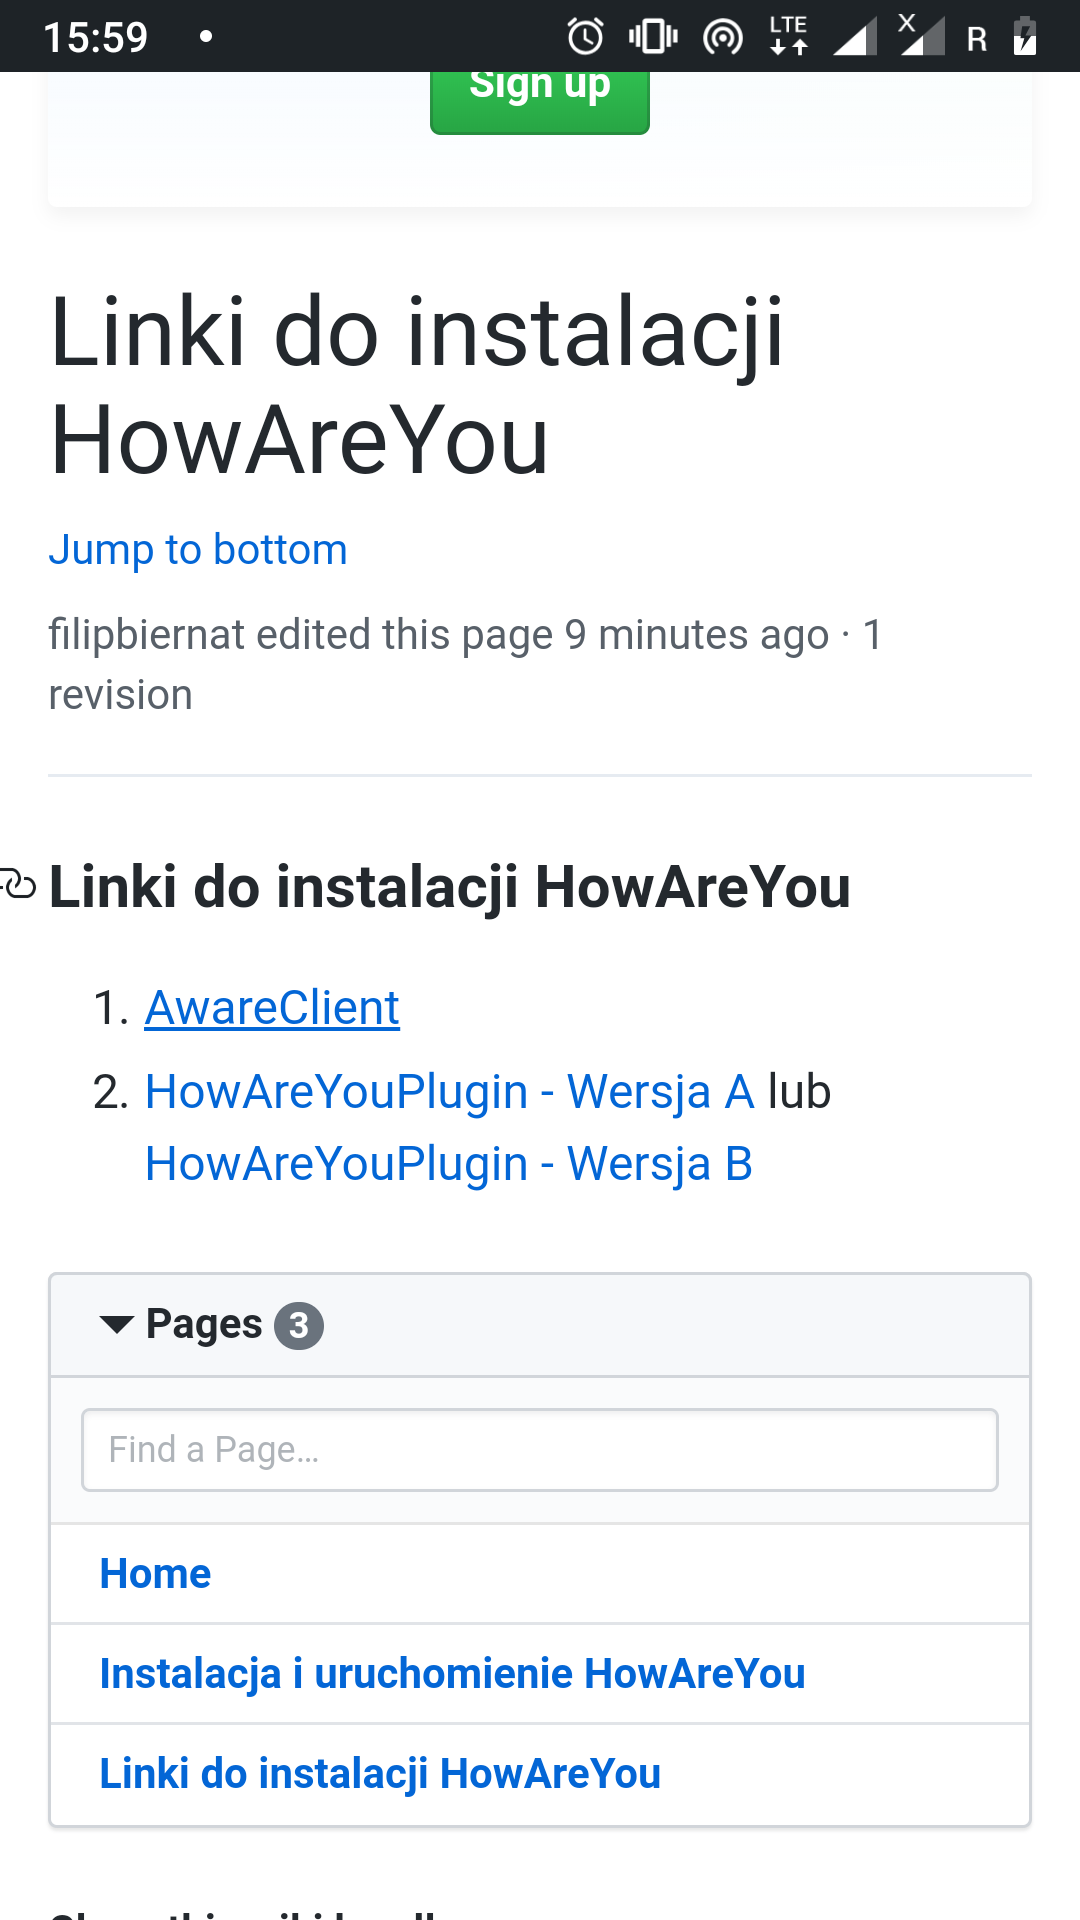
\includegraphics[scale=0.14]{dodatekA/2_1.png}
			\subcaption{\label{subfigure_a}}
		\end{subfigure}
		\begin{subfigure}{0.35\textwidth}
			\centering
			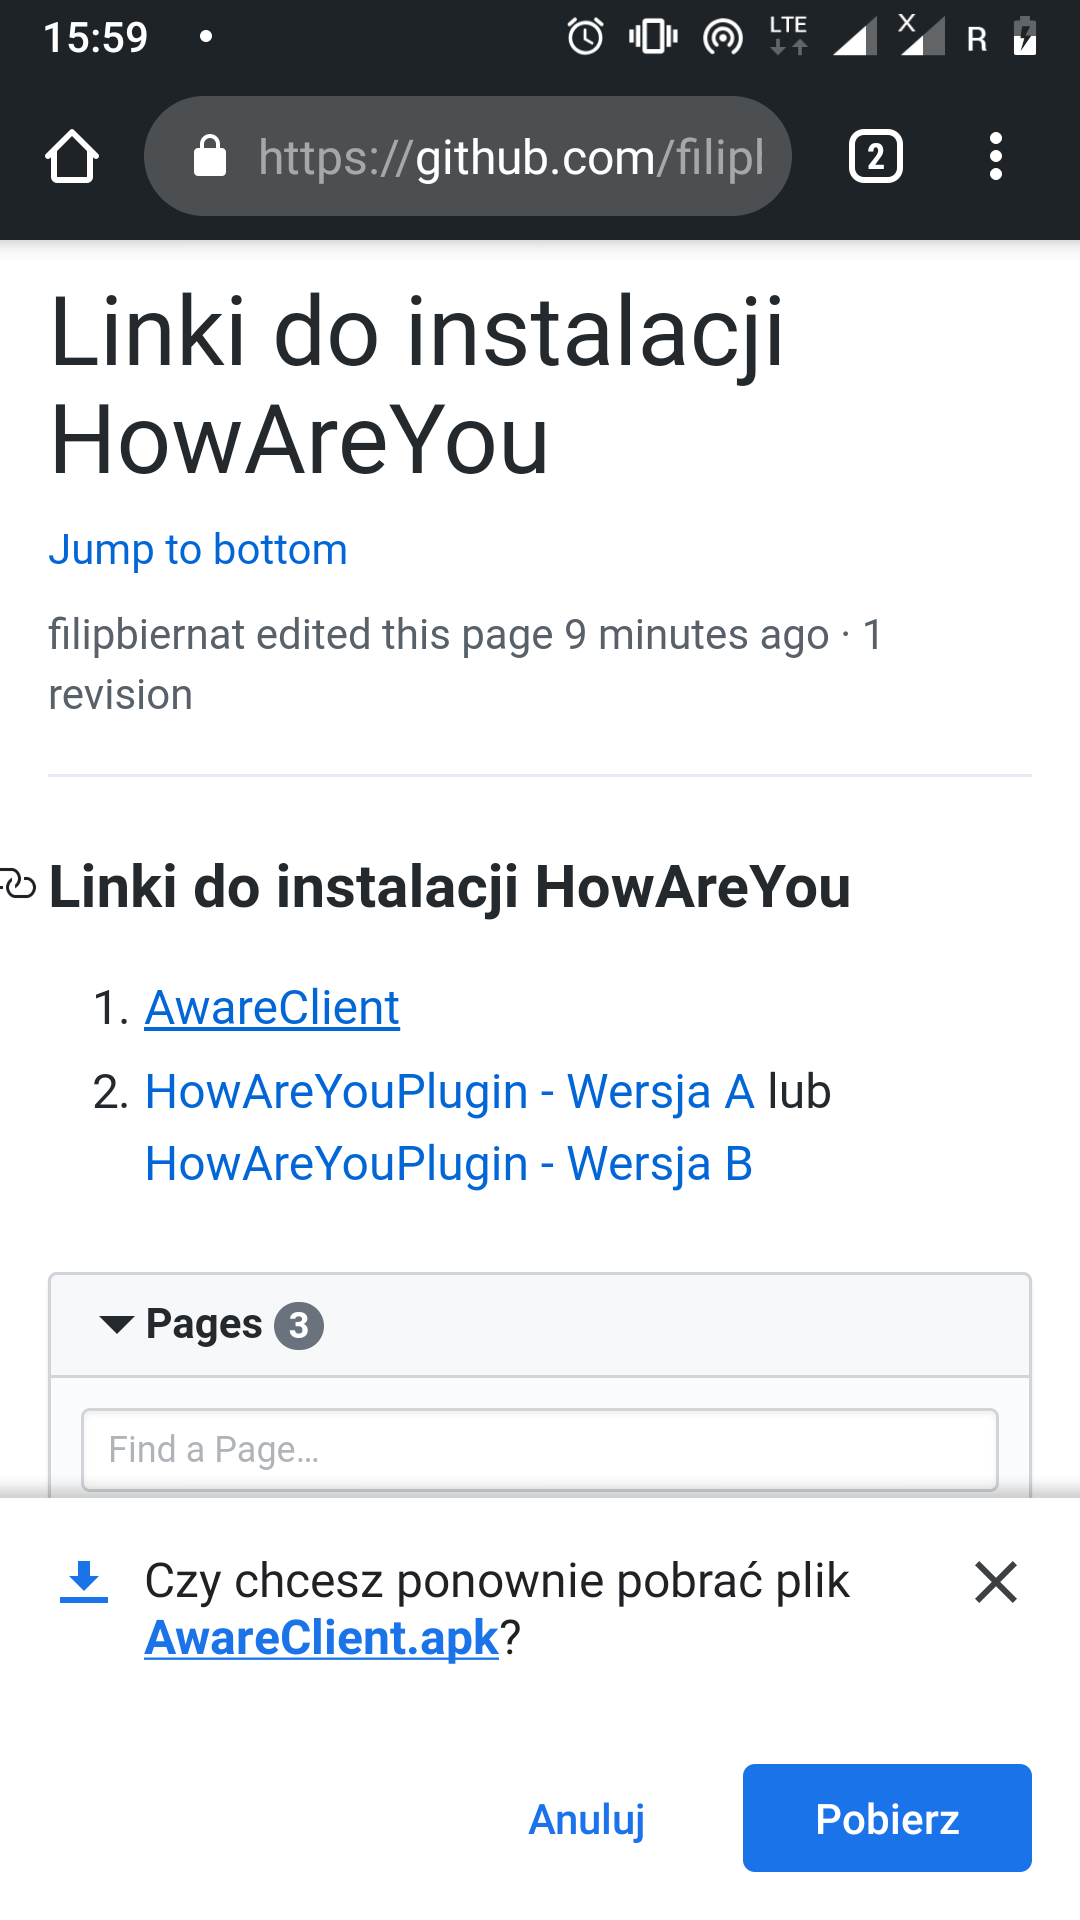
\includegraphics[scale=0.14]{dodatekA/2_2.png}
			\subcaption{\label{subfigure_b}}
		\end{subfigure}
		\caption{ Kroki 1 i 2: Strona www z linkami umożliwiającymi pobranie aplikacji (a) oraz rozpoczęty proces pobierania aplikacji (b).}
	\end{figure}
	\clearpage 
	
	\item Przeglądarka powiadomi Cię o pobraniu pakietu. Kliknij \textit{Otwórz}. 
	
	\item Rozpocznie się instalacja aplikacji. Kliknij \textit{Instaluj}.
	
	\begin{figure}[H]
		\centering
		\begin{subfigure}{0.35\textwidth}
			\centering
			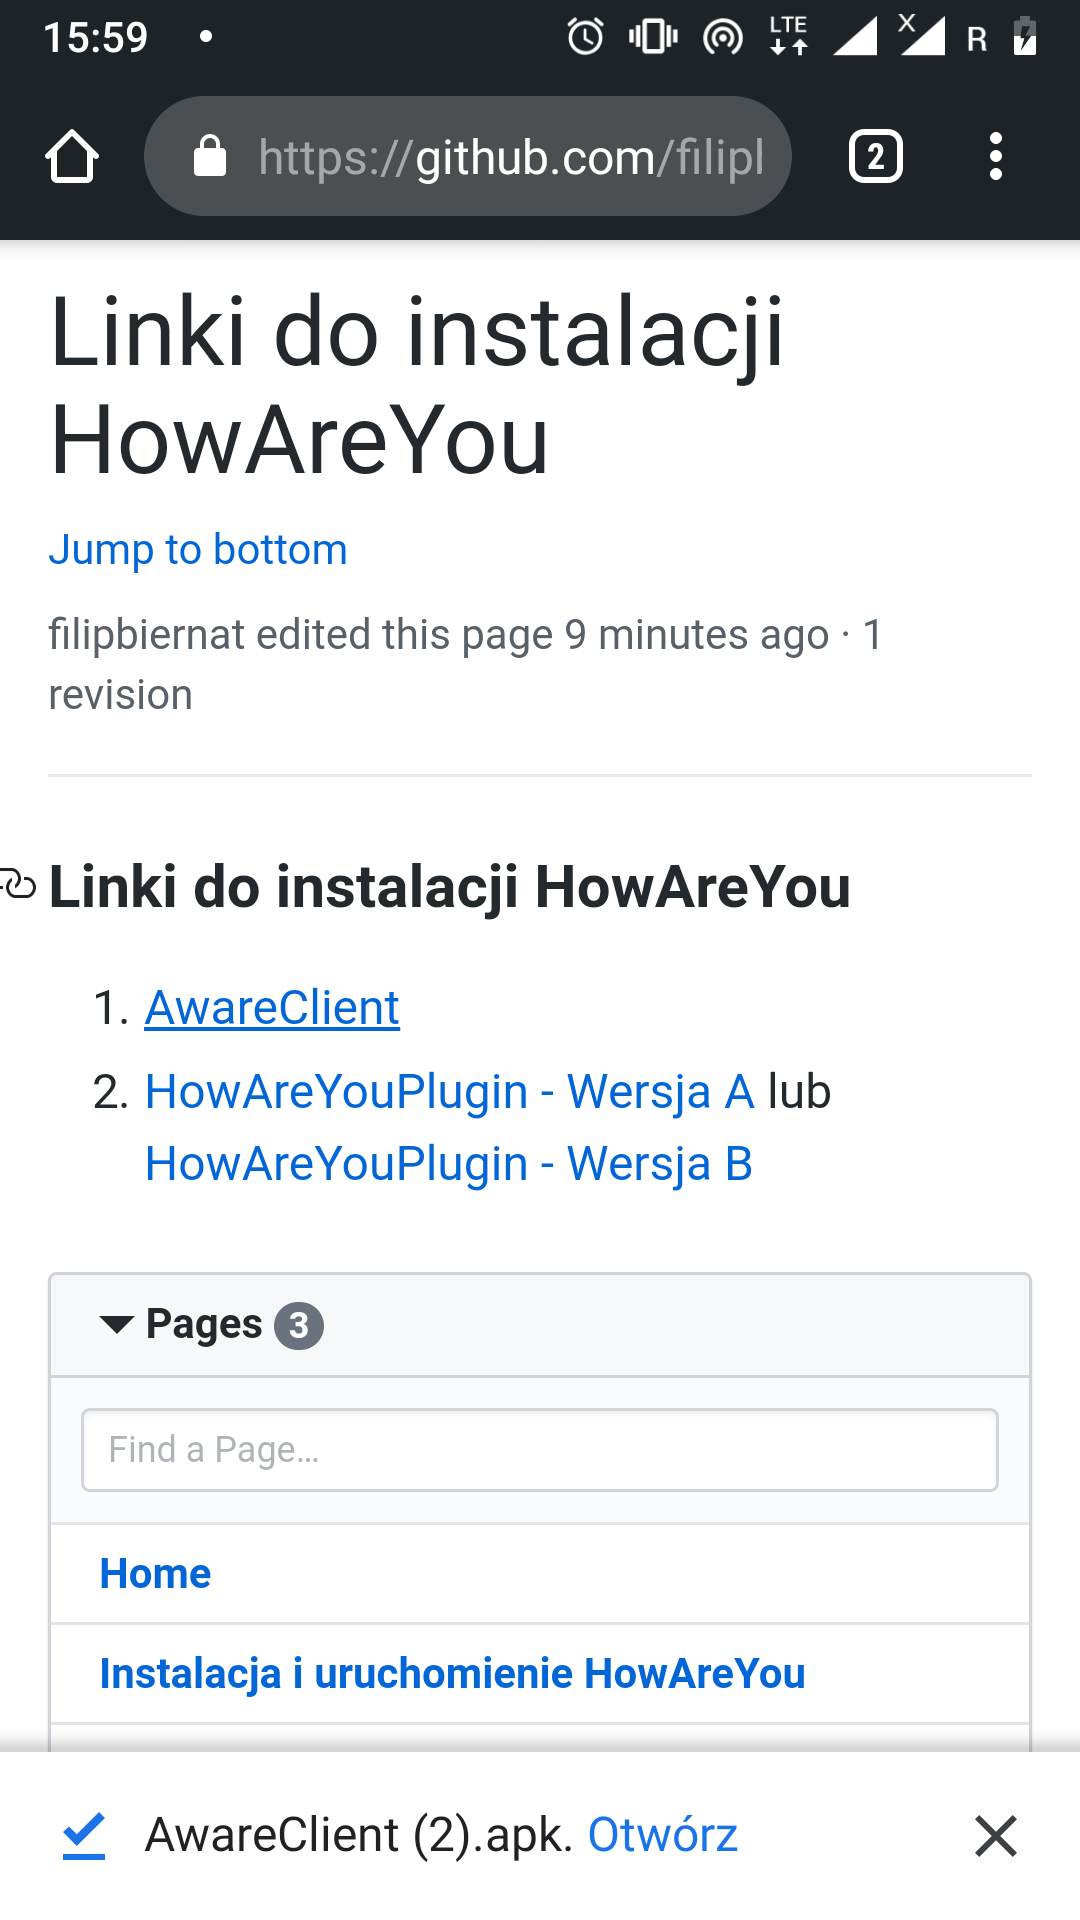
\includegraphics[scale=0.14]{dodatekA/2_3.png}
			\subcaption{\label{subfigure_a}}
		\end{subfigure}
		\begin{subfigure}{0.35\textwidth}
			\centering
			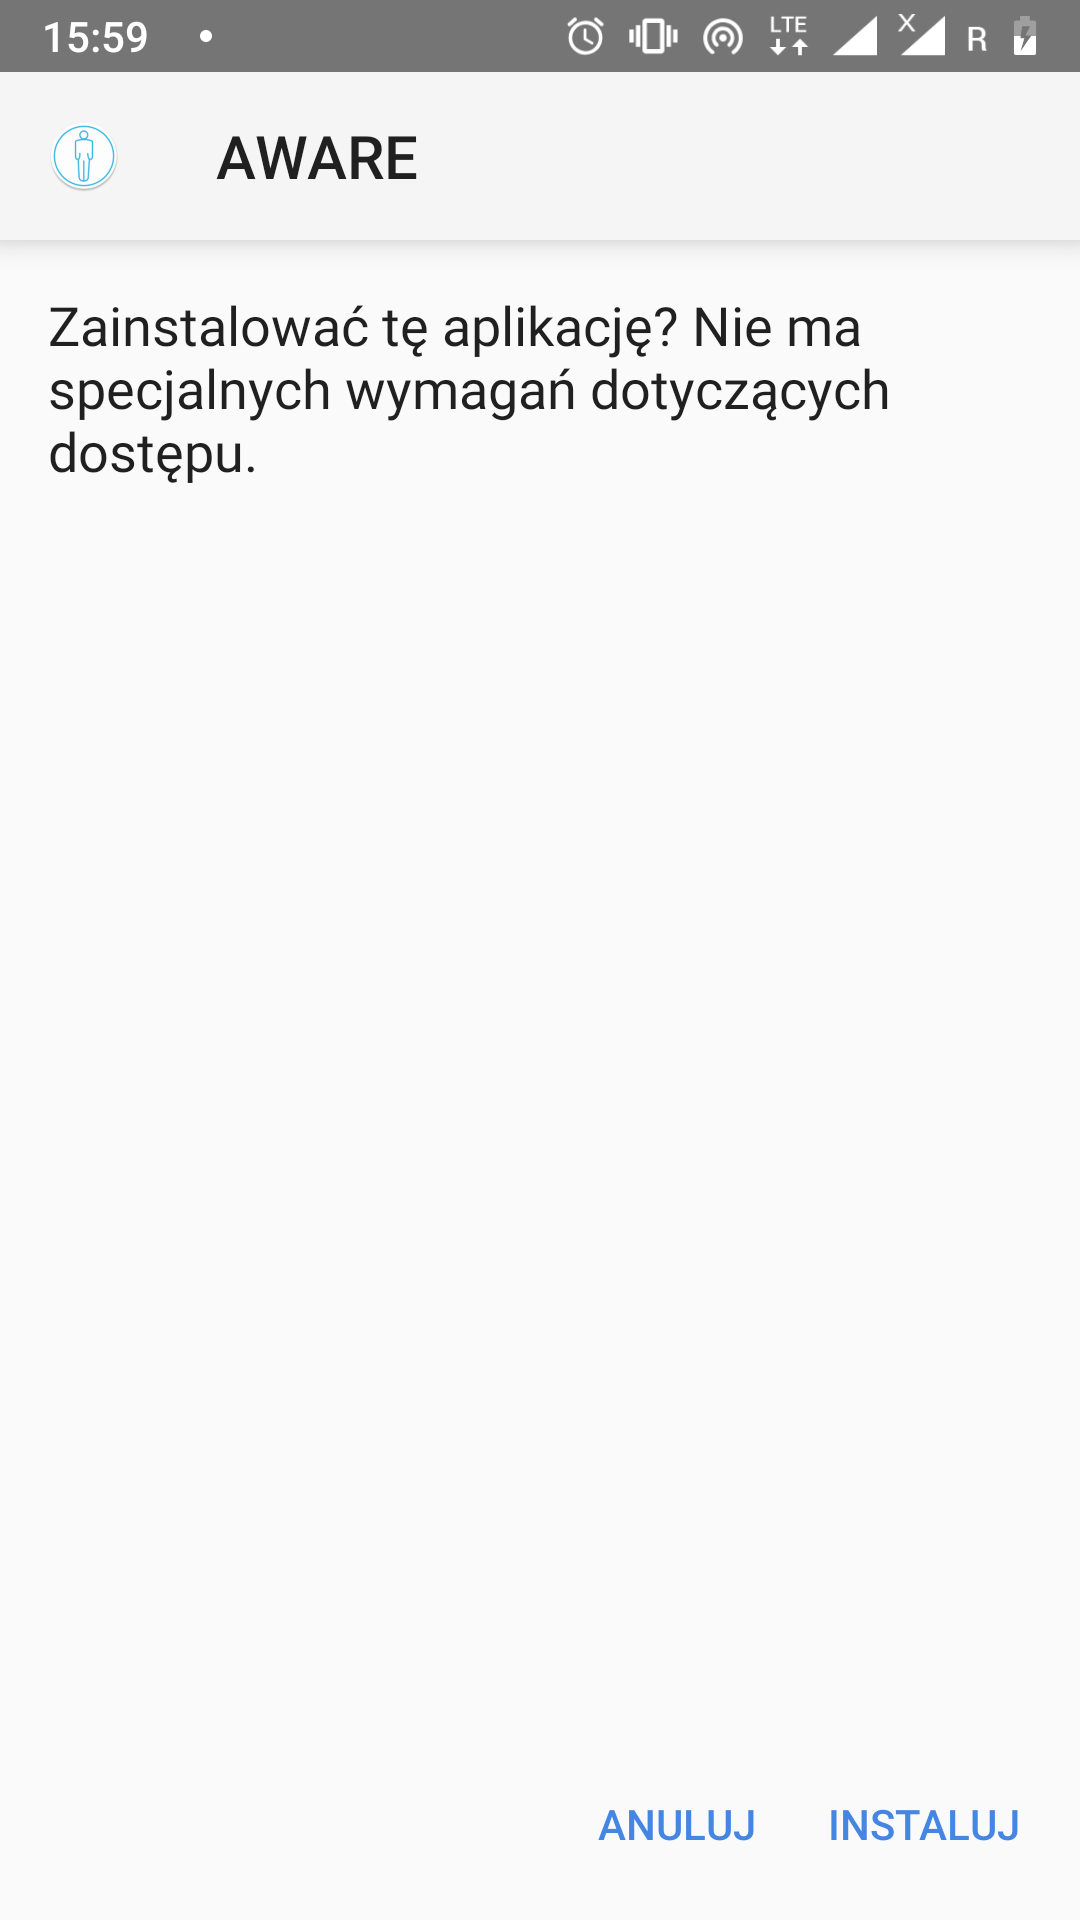
\includegraphics[scale=0.14]{dodatekA/2_4.png}
			\subcaption{\label{subfigure_b}}
		\end{subfigure}
		\caption{ Kroki 3 i 4: Wybór przycisków \textit{Otwórz} (a) oraz \textit{Instaluj} (b).}
	\end{figure}
	\clearpage 
	
	\item Po zakończeniu instalacji kliknij \textit{Gotowe} i powróć do przeglądarki.
	
	\item Przed rozpoczęciem badania zostałeś poproszony o pobranie wersji A lub wersji B aplikacji. Upewnij się którą wersję powinieneś wykorzystać.
	
	\item Pobierz plik instalatora klikając na \textit{HowAreYouPlugin - Wersja A} lub \textit{HowAreYouPlugin - Wersja B}.
	
	\begin{figure}[H]
		\centering
		\begin{subfigure}{0.35\textwidth}
			\centering
			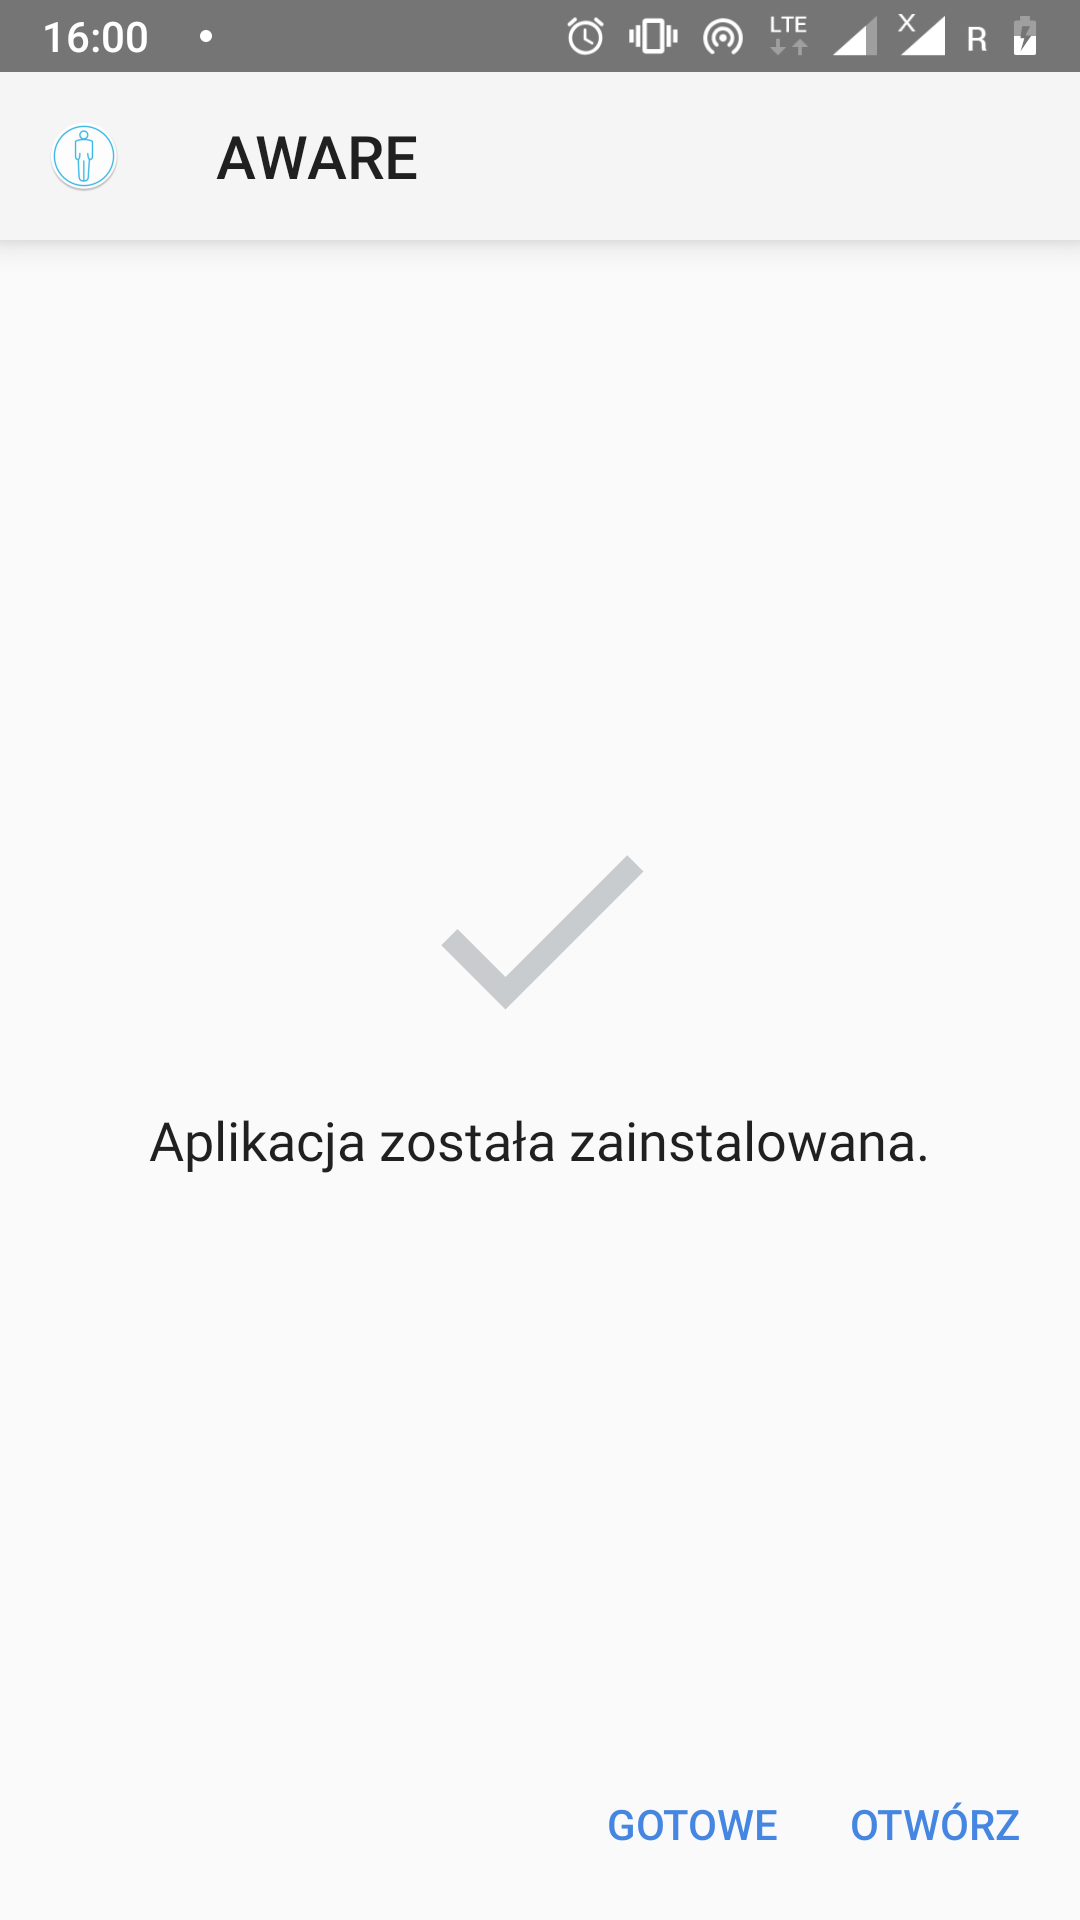
\includegraphics[scale=0.14]{dodatekA/2_5.png}
			\subcaption{\label{subfigure_a}}
		\end{subfigure}
		\begin{subfigure}{0.35\textwidth}
			\centering
			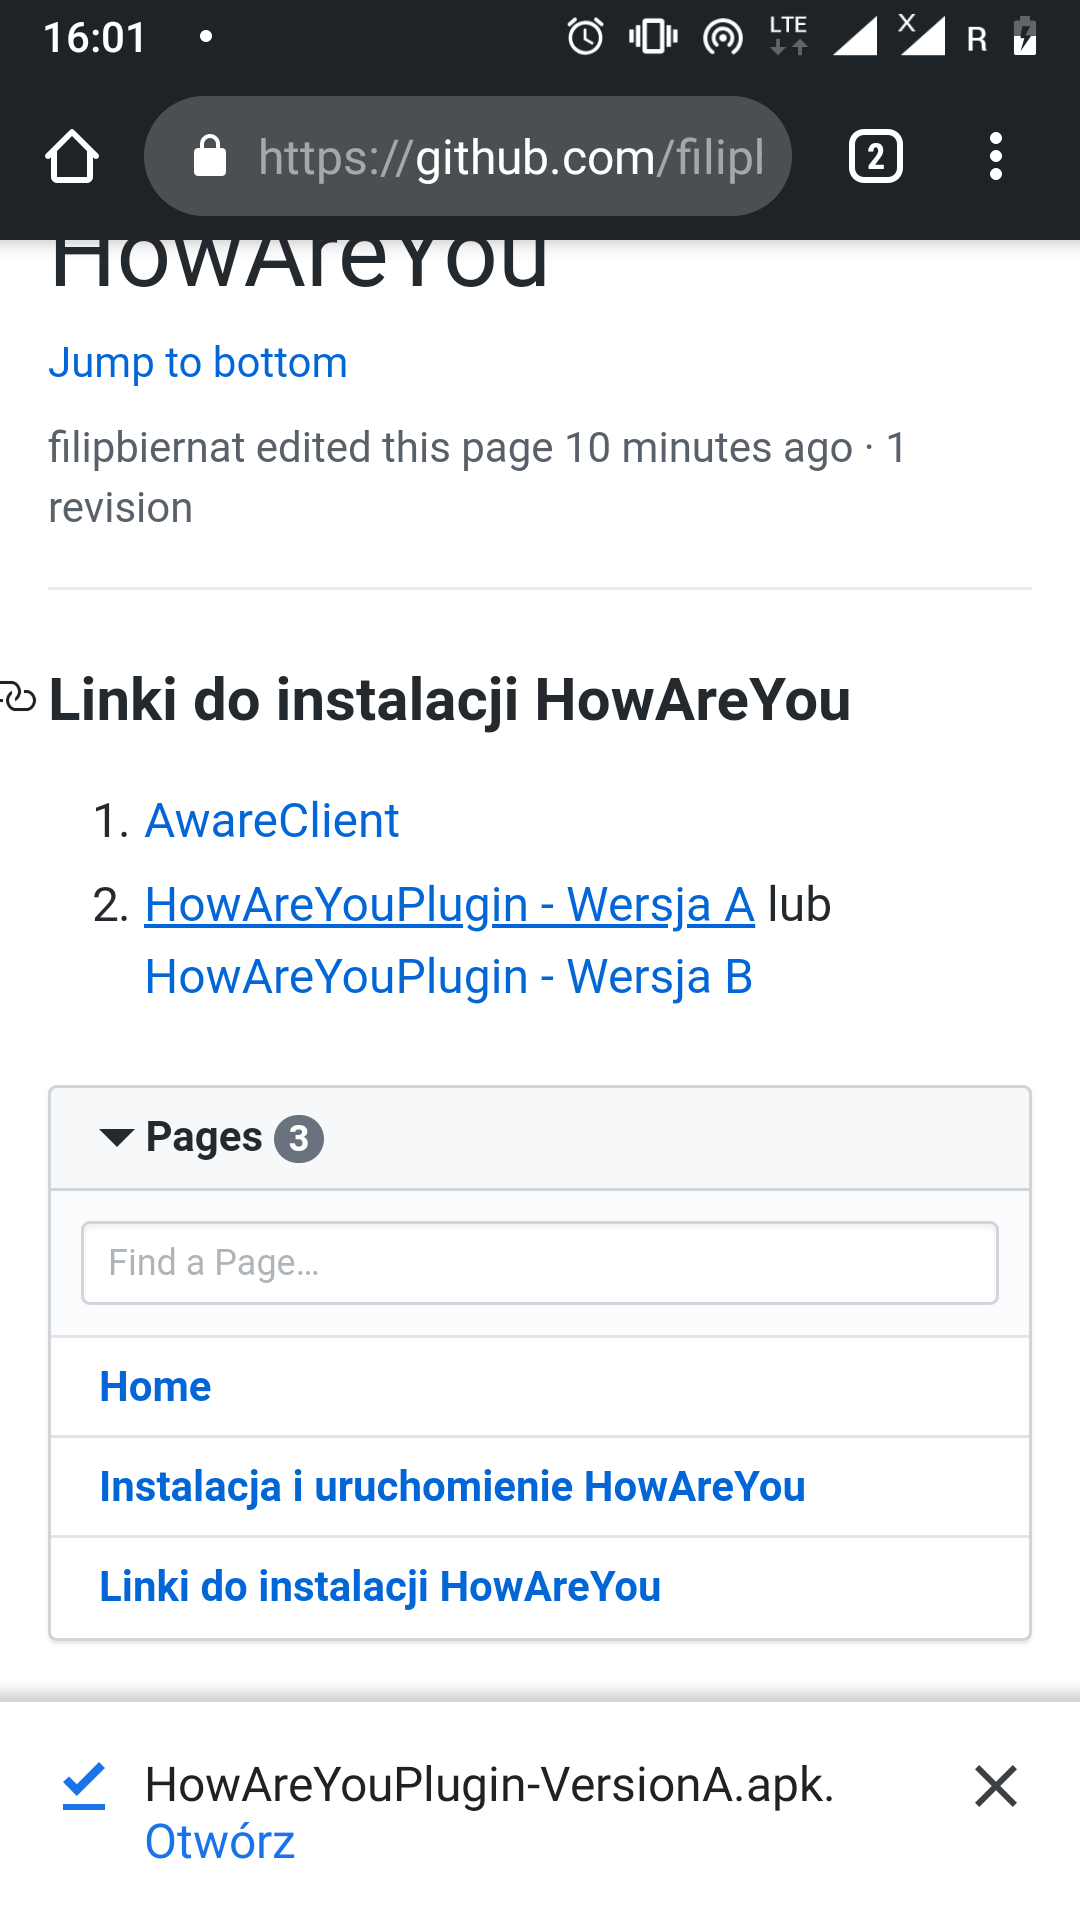
\includegraphics[scale=0.14]{dodatekA/2_7.png}
			\subcaption{\label{subfigure_b}}
		\end{subfigure}
		\caption{ Kroki 5 i 7: Wybór przycisku \textit{Gotowe} (a) oraz wybór wersji pluginu (b).}
	\end{figure}
	\clearpage 
	
	\item Podobnie jak wcześniej, kliknij \textit{Otwórz}. Rozpocznie się instalacja aplikacji. Kliknij \textit{Instaluj}. 
	
	\item Ponownie kliknij przycisk \textit{Gotowe}. Zamknij przeglądarkę i powróć do ekranu głównego.
	
	\begin{figure}[H]
		\centering
		\begin{subfigure}{0.35\textwidth}
			\centering
			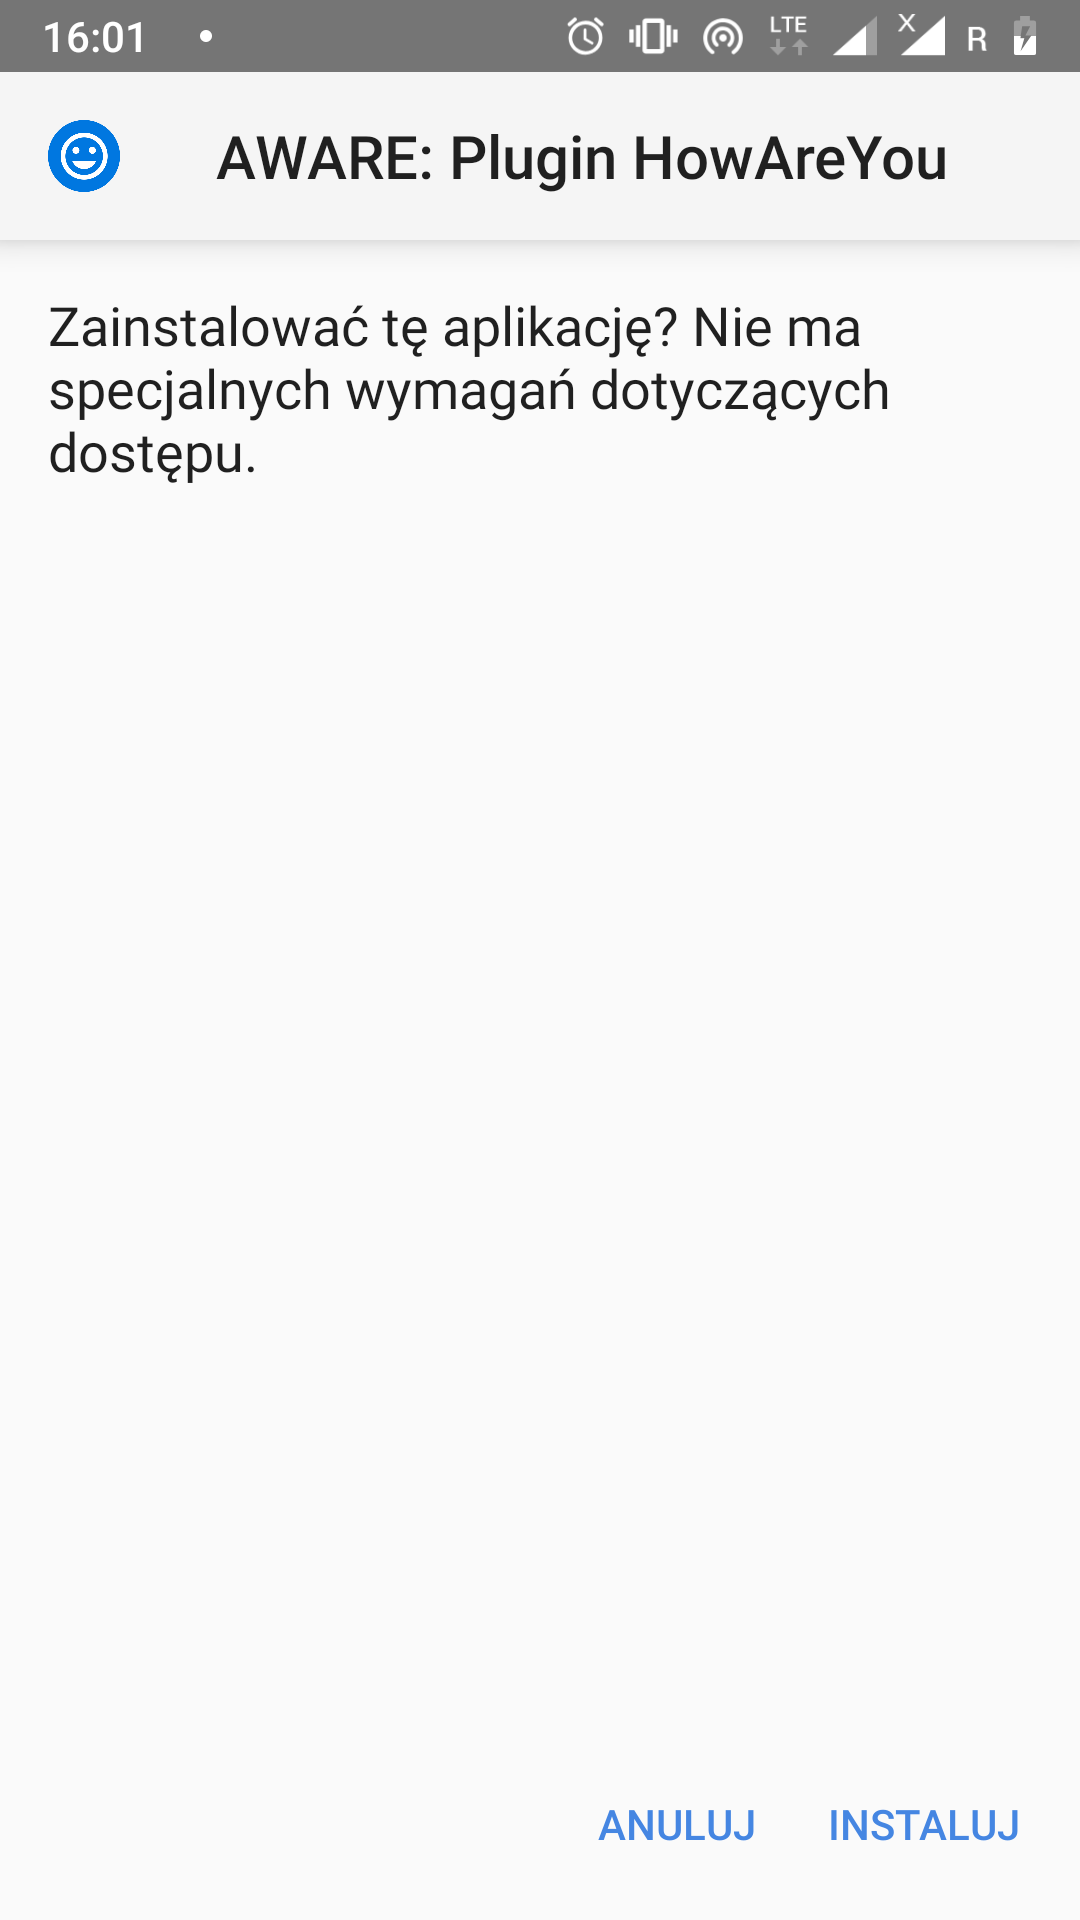
\includegraphics[scale=0.14]{dodatekA/2_8.png}
			\subcaption{\label{subfigure_a}}
		\end{subfigure}
		\begin{subfigure}{0.35\textwidth}
			\centering
			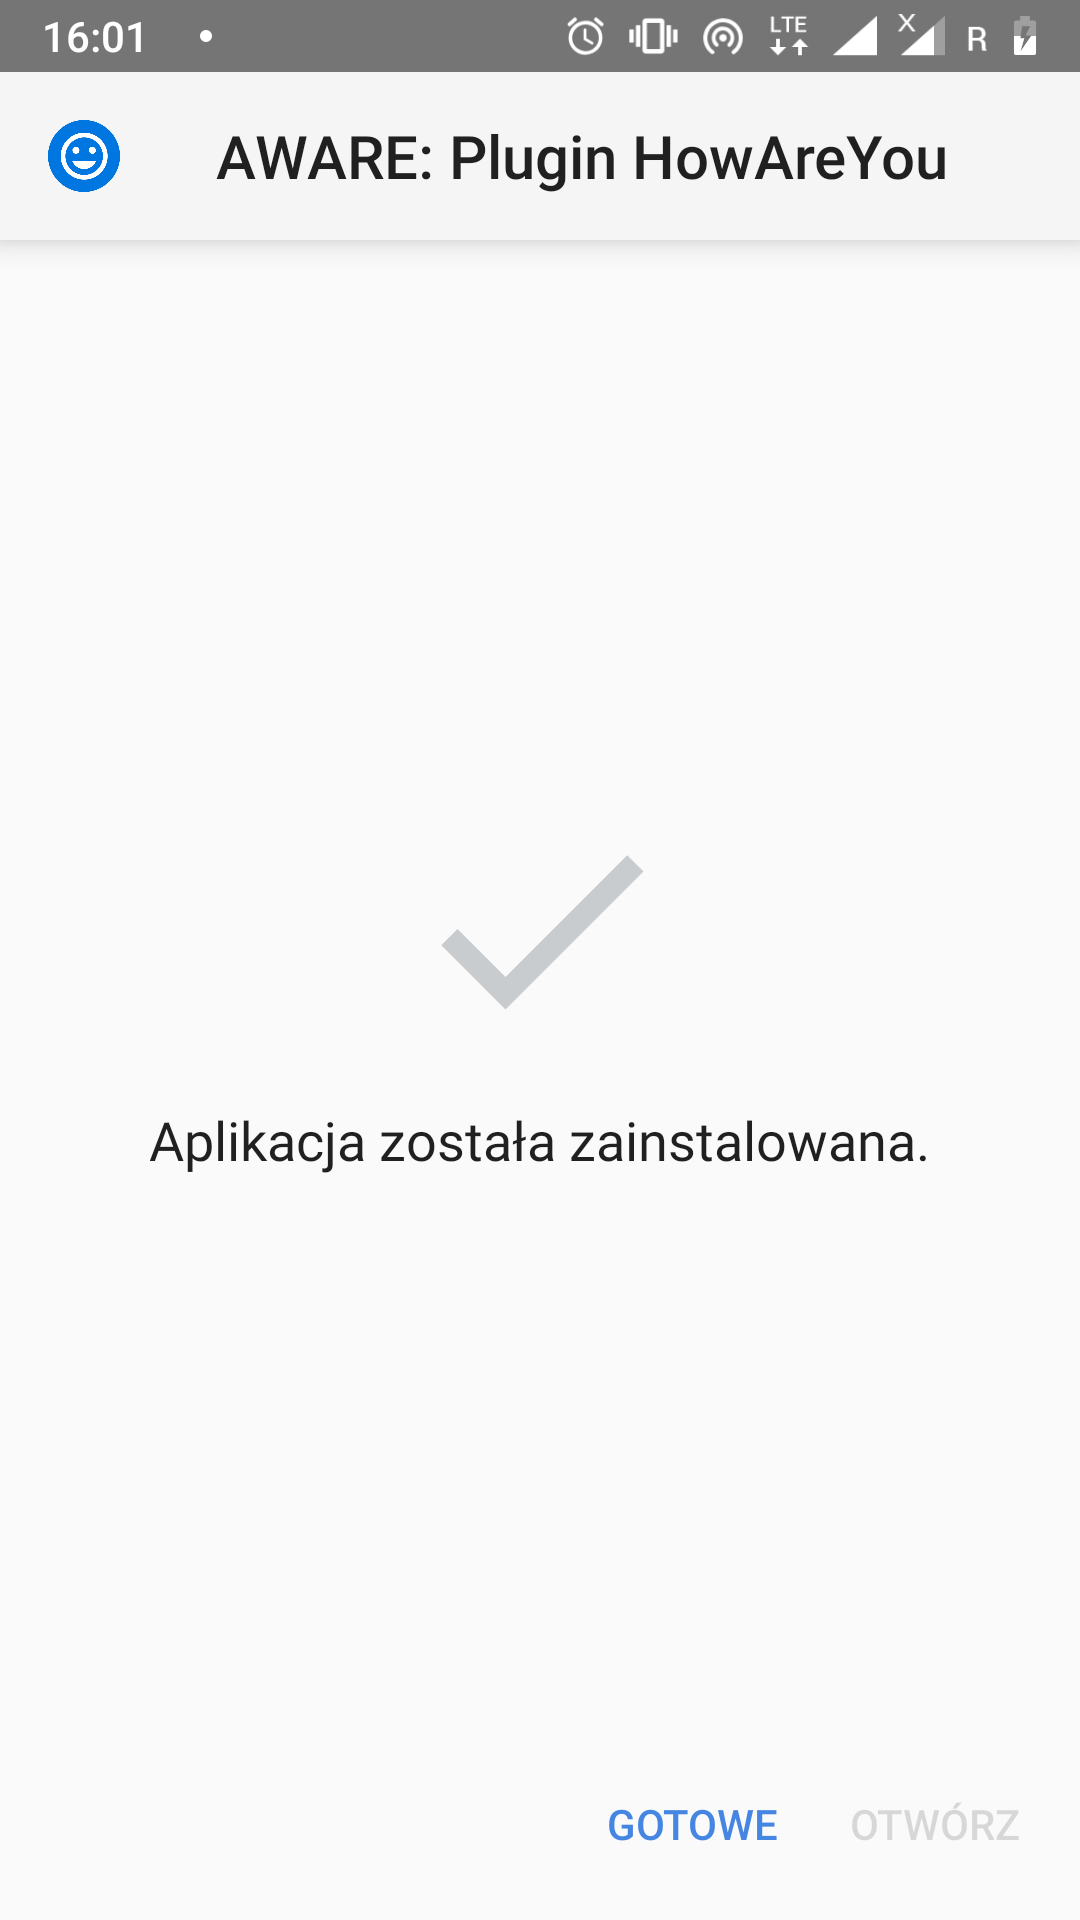
\includegraphics[scale=0.14]{dodatekA/2_9.png}
			\subcaption{\label{subfigure_b}}
		\end{subfigure}
		\caption{ Kroki 8 i 9: Wybór przycisków \textit{Instaluj} (a) oraz \textit{Gotowe} (b).}
	\end{figure}
	\clearpage 
	
\end{enumerate}

%---------------------------------------------------------------------------

\section{Etap 3: Konfiguracja aplikacji}
\label{sec:pobranieIInstalacjaAplikacji}

Ostatnim krokiem będzie konfiguracja aplikacji klietna oraz pluginu \textit{HowAreYou}.

\begin{enumerate}
	
	\item Uruchom aplikację \textit{AWARE}.
	
	\item Zostaniesz zapytany o zgody na wykorzystanie zasobów telefonu. Zatwierdź odpowiednie zgody.
	
	\begin{figure}[H]
		\centering
		\begin{subfigure}{0.35\textwidth}
			\centering
			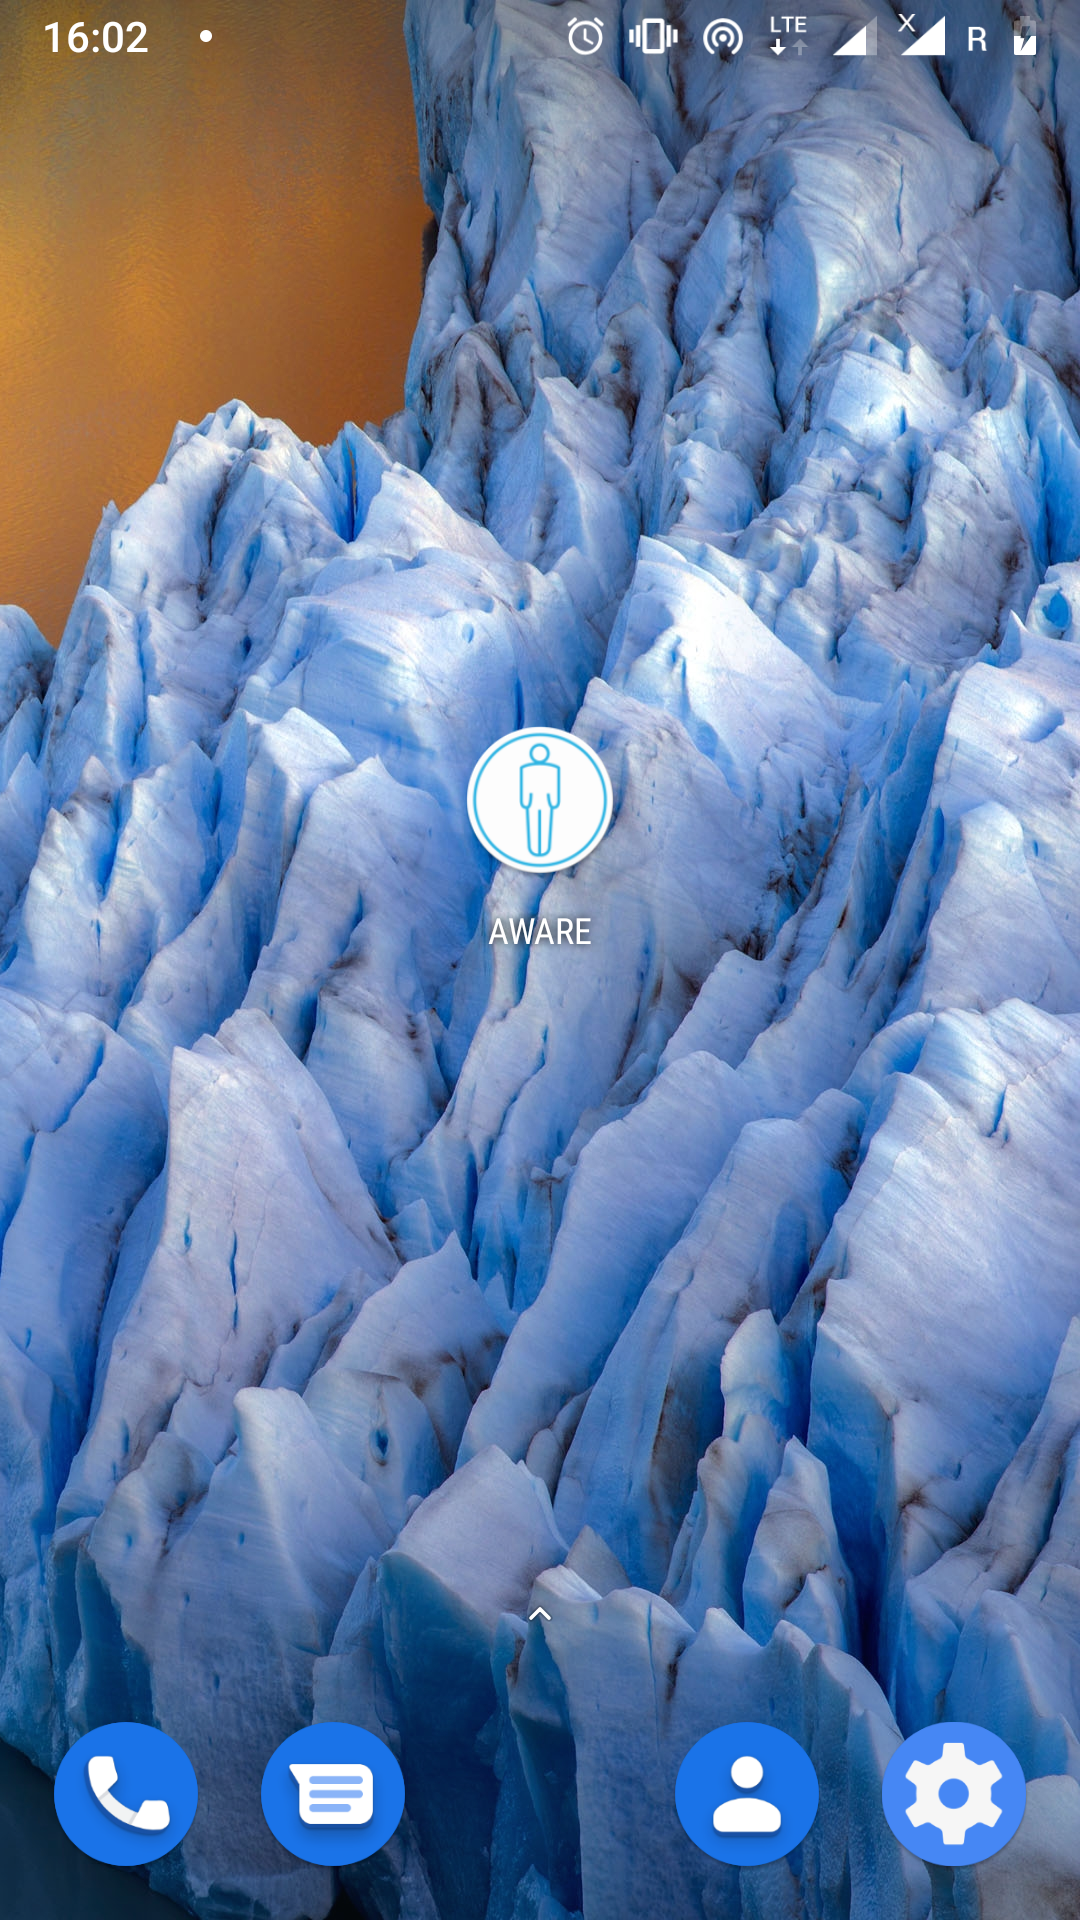
\includegraphics[scale=0.14]{dodatekA/3_1.png}
			\subcaption{\label{subfigure_a}}
		\end{subfigure}
		\begin{subfigure}{0.35\textwidth}
			\centering
			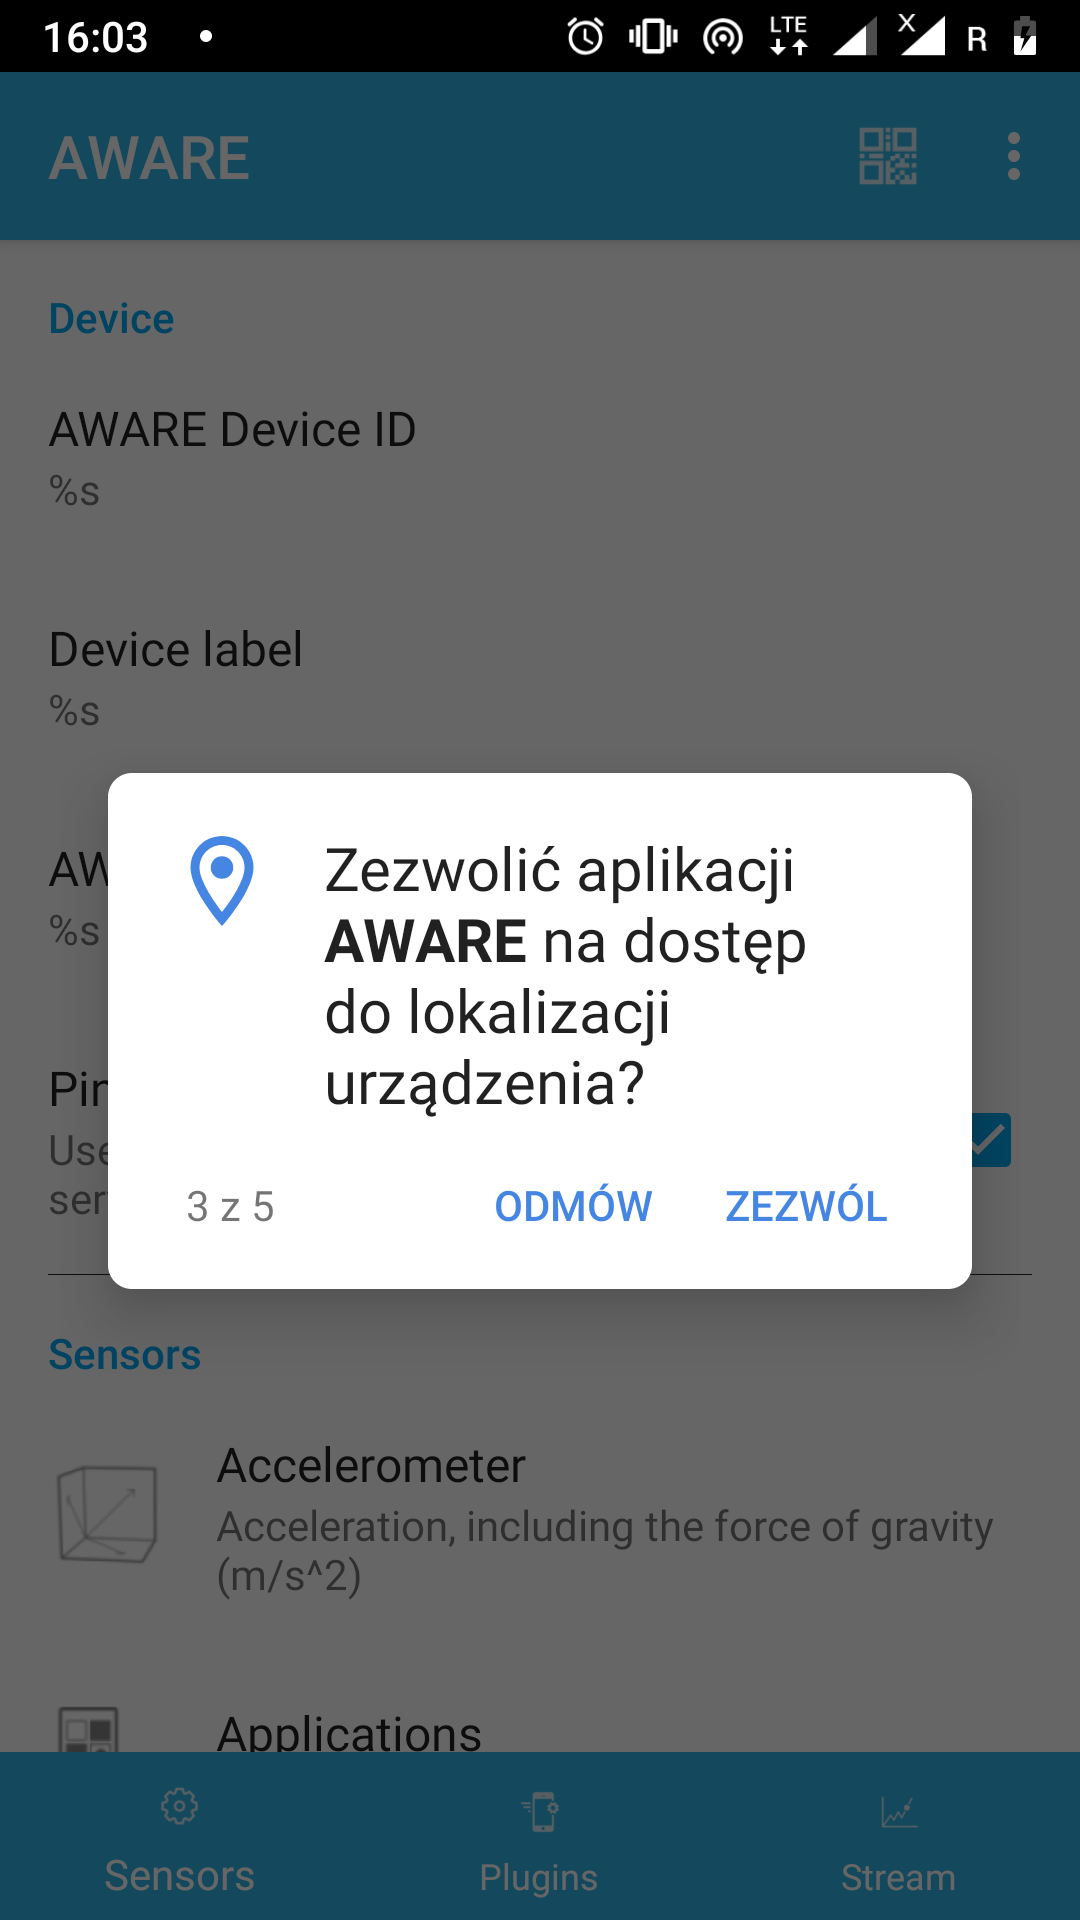
\includegraphics[scale=0.14]{dodatekA/3_2.png}
			\subcaption{\label{subfigure_b}}
		\end{subfigure}
		\caption{ Kroki 1 i 2: Uruchomienie aplikacji \textit{AWARE} (a) oraz widok zapytania użytkownika o zgodę (b).}
	\end{figure}
	\clearpage 
	
	\item W aplikacji przejdź do zakładki \textit{Plugins}.
	
	\item Wybierz plugin \textit{HowAreYou}. Jeżeli plugin nie jest jeszcze aktywny, kliknij \textit{Activate}.
	
	\begin{figure}[H]
		\centering
		\begin{subfigure}{0.35\textwidth}
			\centering
			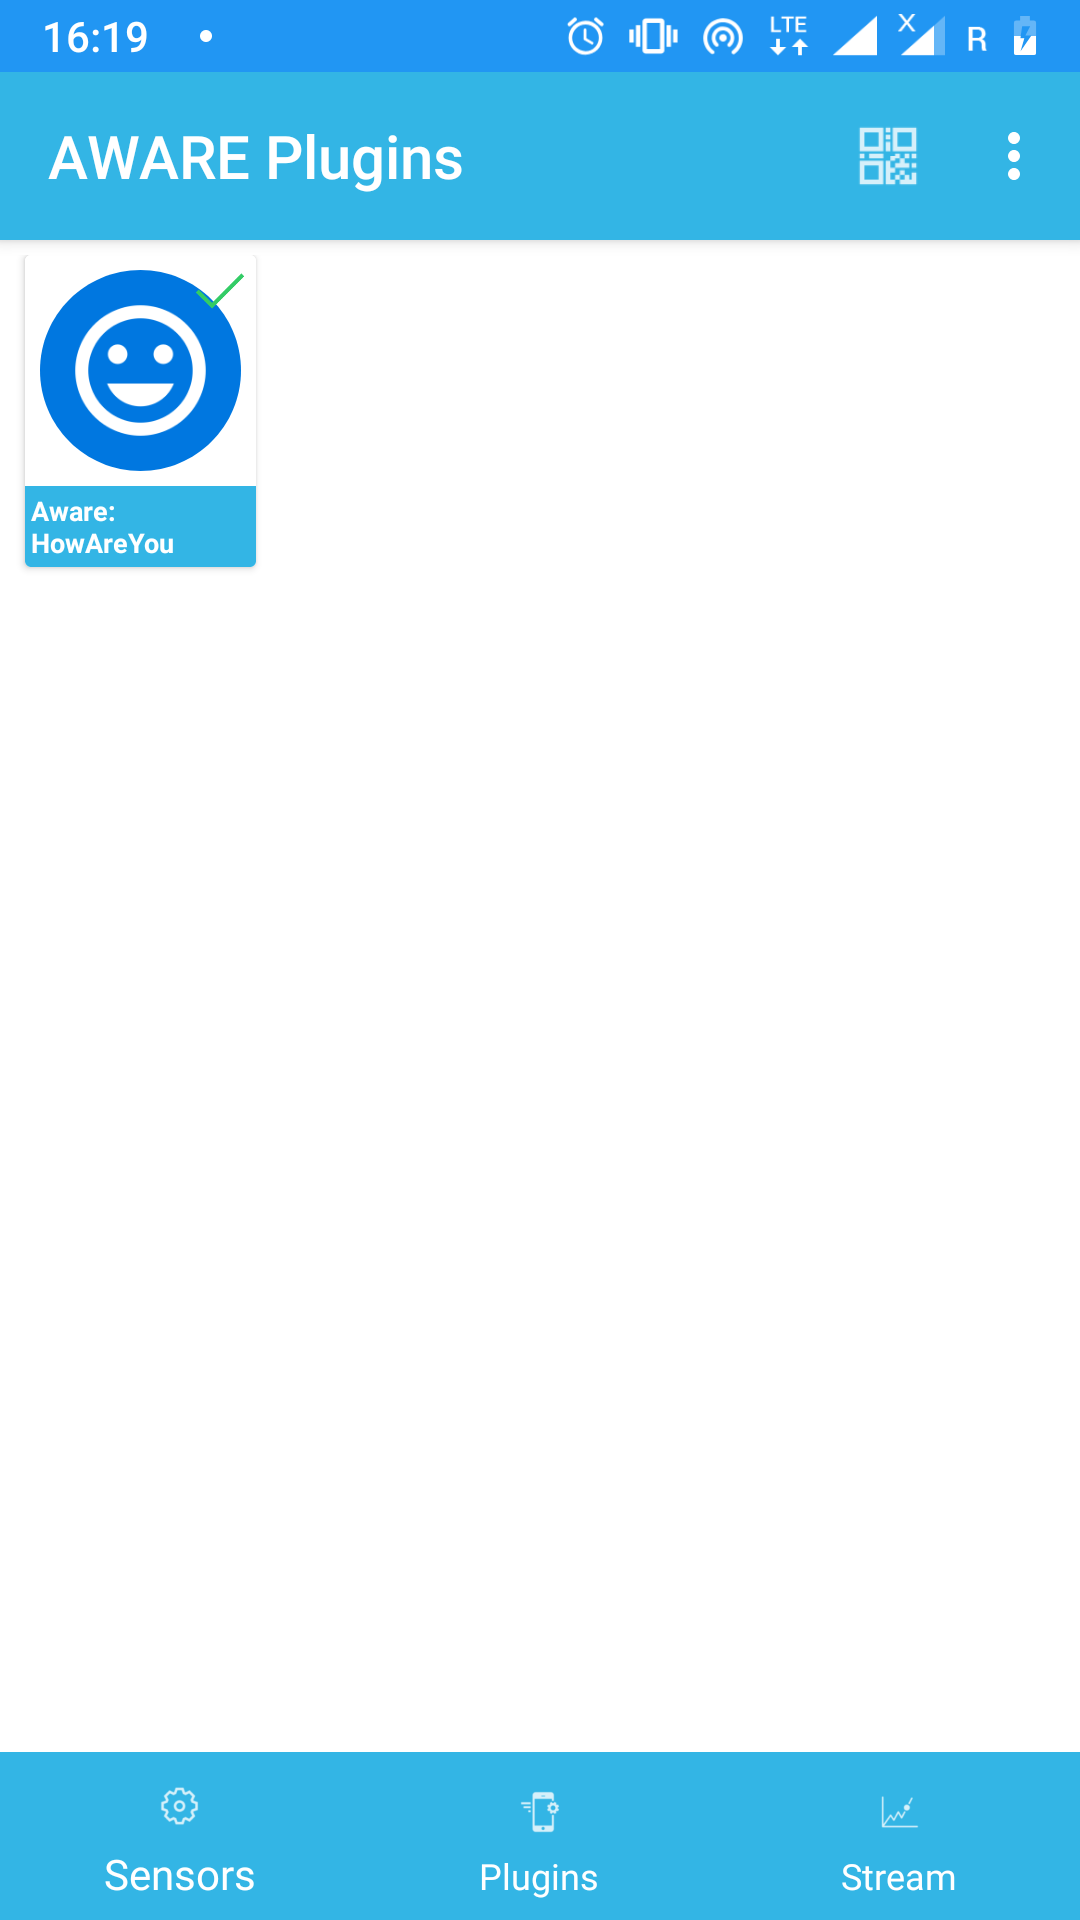
\includegraphics[scale=0.14]{dodatekA/3_3.png}
			\subcaption{\label{subfigure_a}}
		\end{subfigure}
		\begin{subfigure}{0.35\textwidth}
			\centering
			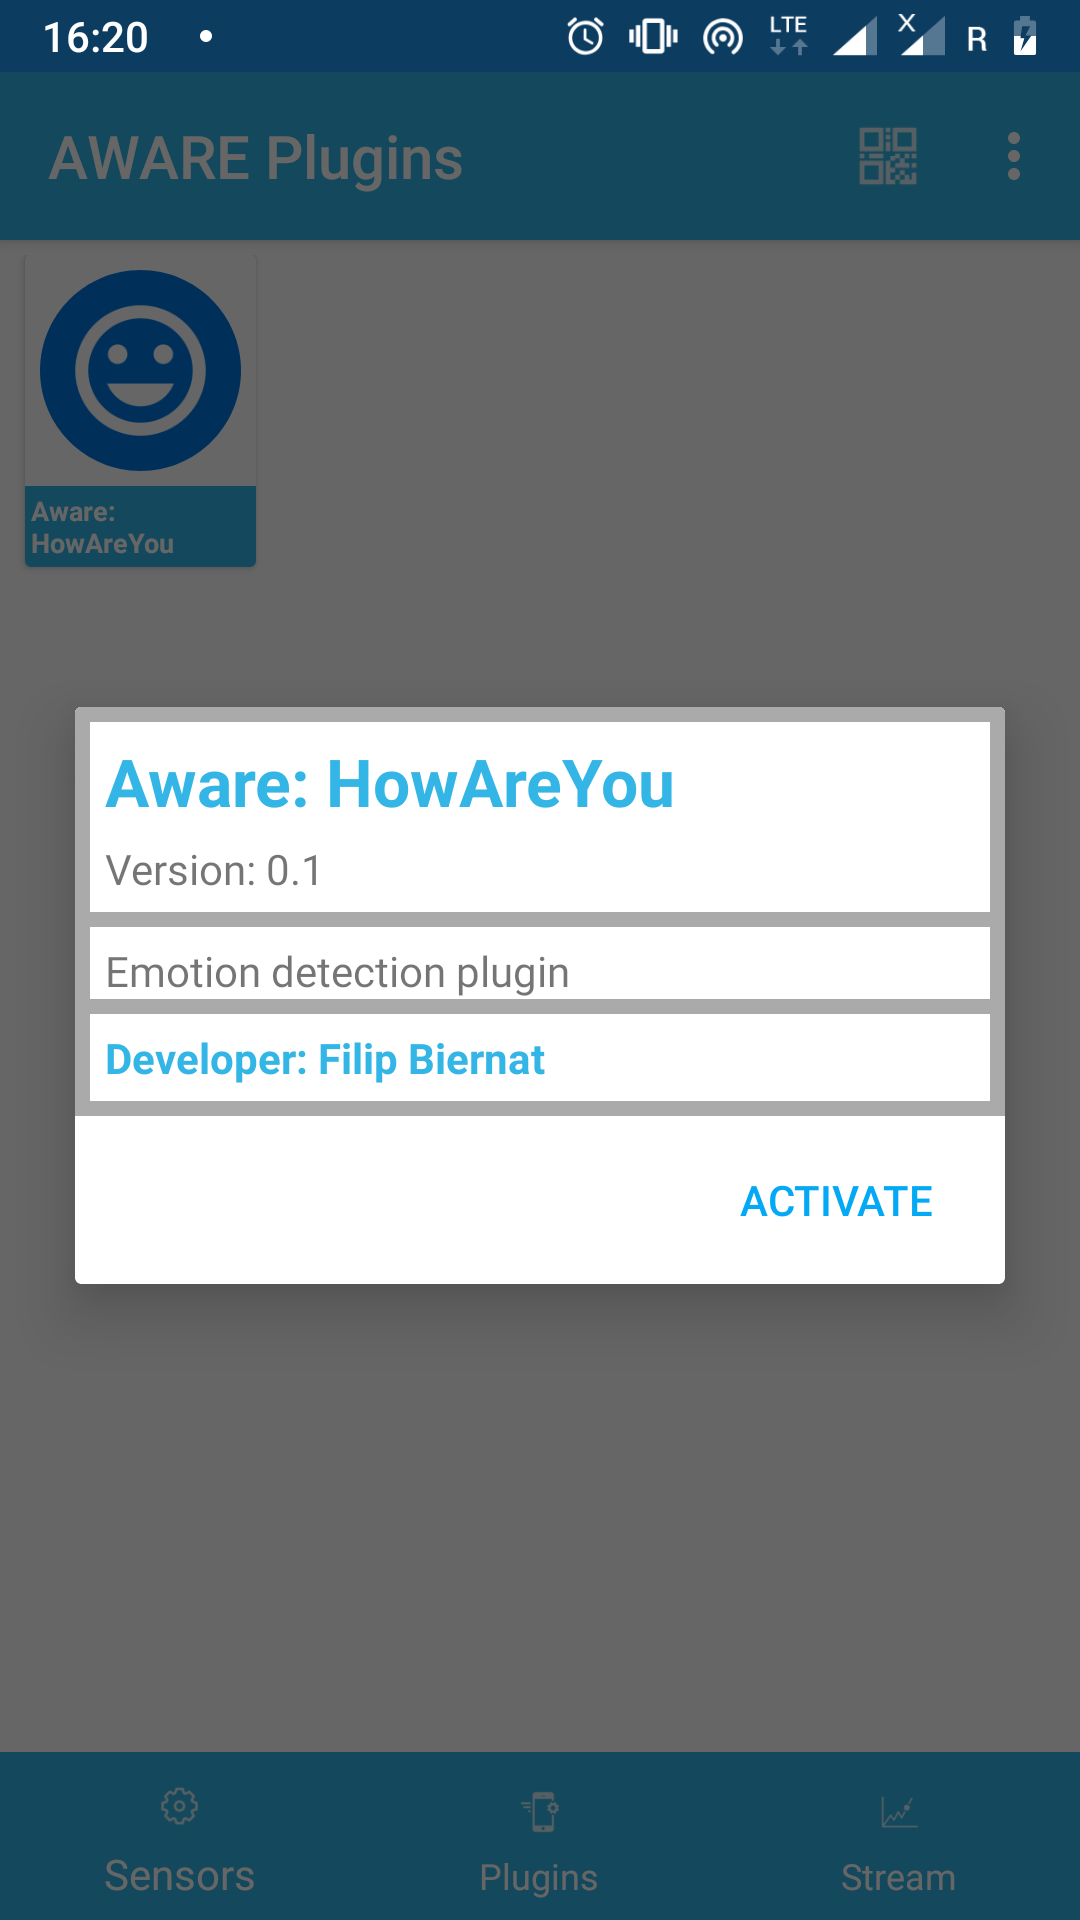
\includegraphics[scale=0.14]{dodatekA/3_4.png}
			\subcaption{\label{subfigure_b}}
		\end{subfigure}
		\caption{ Kroki 3 i 4: Widok listy dostępnych pluginów (a) oraz menu aktywacji pluginu (b).}
	\end{figure}
	\clearpage 
	
	\item Zostaniesz zapytany o zgody na wykorzystanie zasobów telefonu. Zatwierdź odpowiednie zgody.
	
	\item W systemie pojawi się powiadomienie \textit{Please enable AWARE}. Kliknij na obszar powiadomienia. Otworzy się okno \textit{Accessibility Service}.
	
	\begin{figure}[H]
		\centering
		\begin{subfigure}{0.35\textwidth}
			\centering
			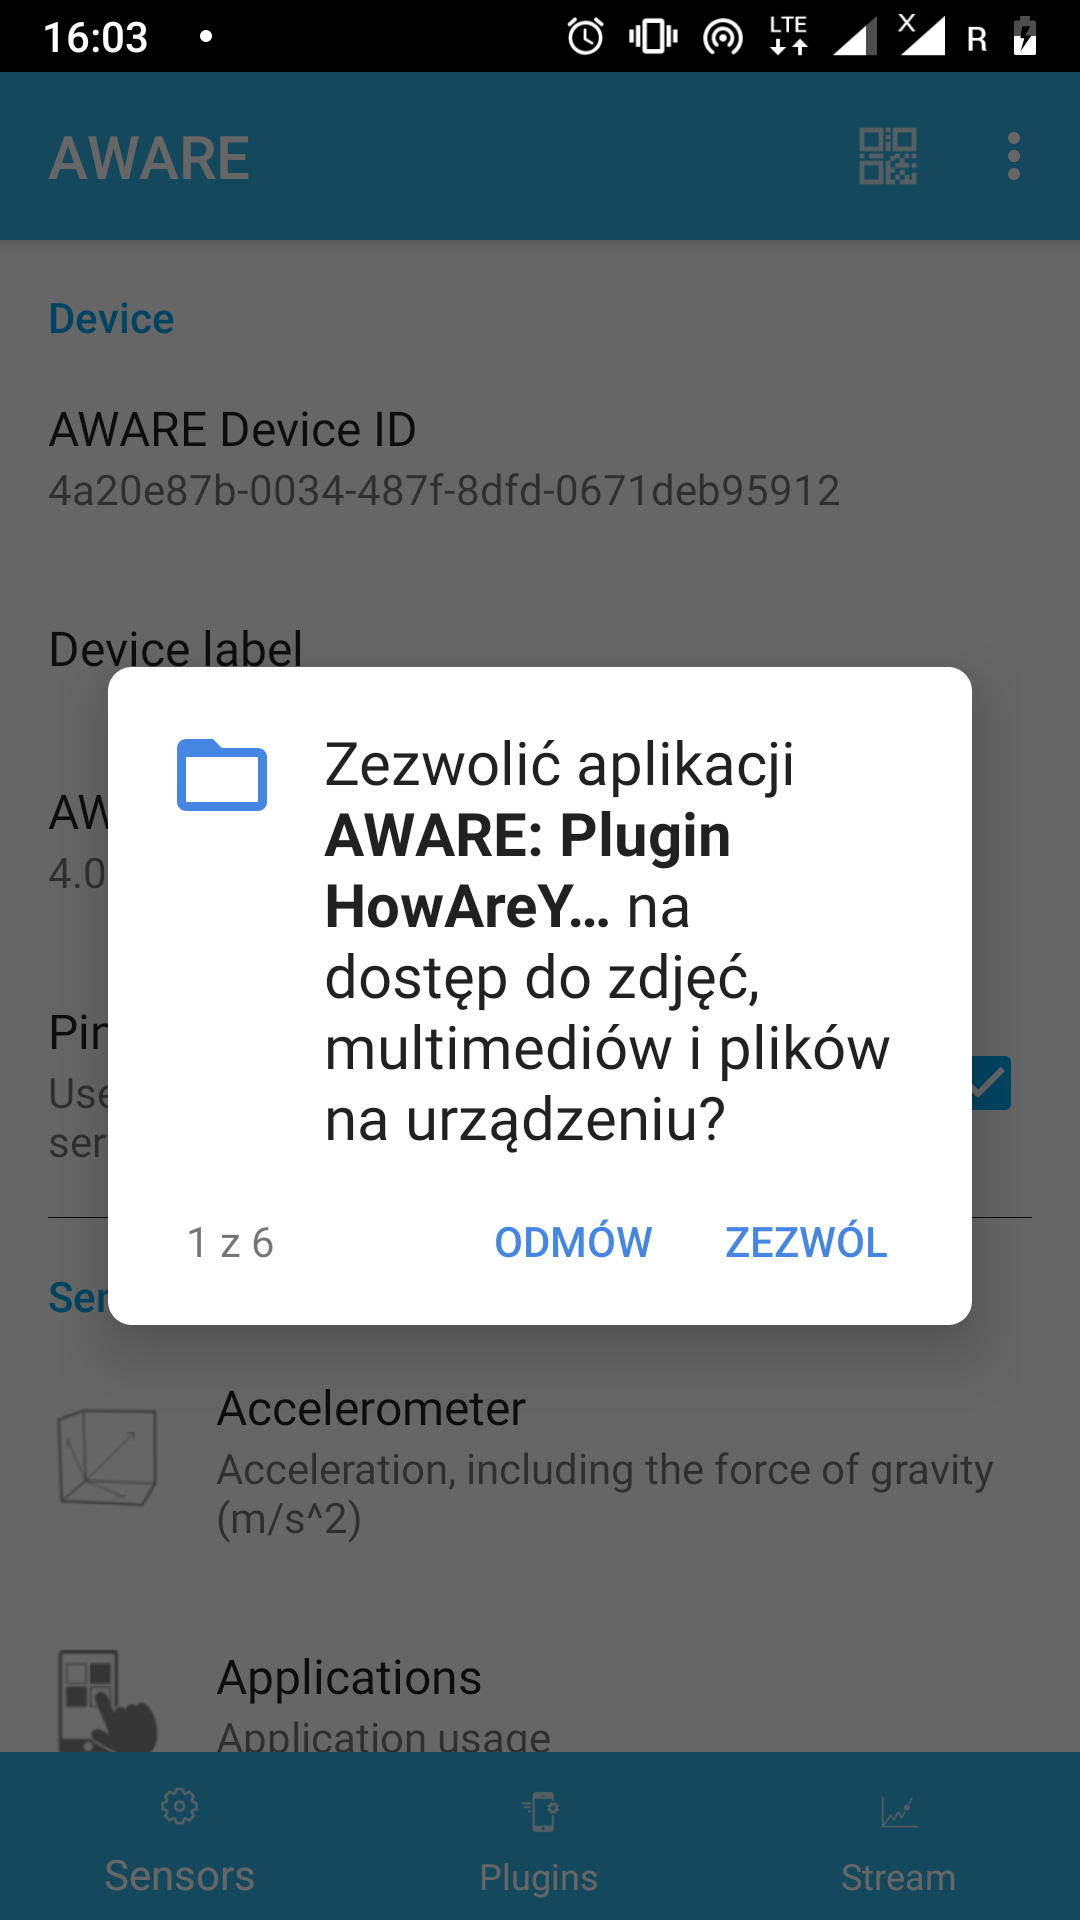
\includegraphics[scale=0.14]{dodatekA/3_5.png}
			\subcaption{\label{subfigure_a}}
		\end{subfigure}
		\begin{subfigure}{0.35\textwidth}
			\centering
			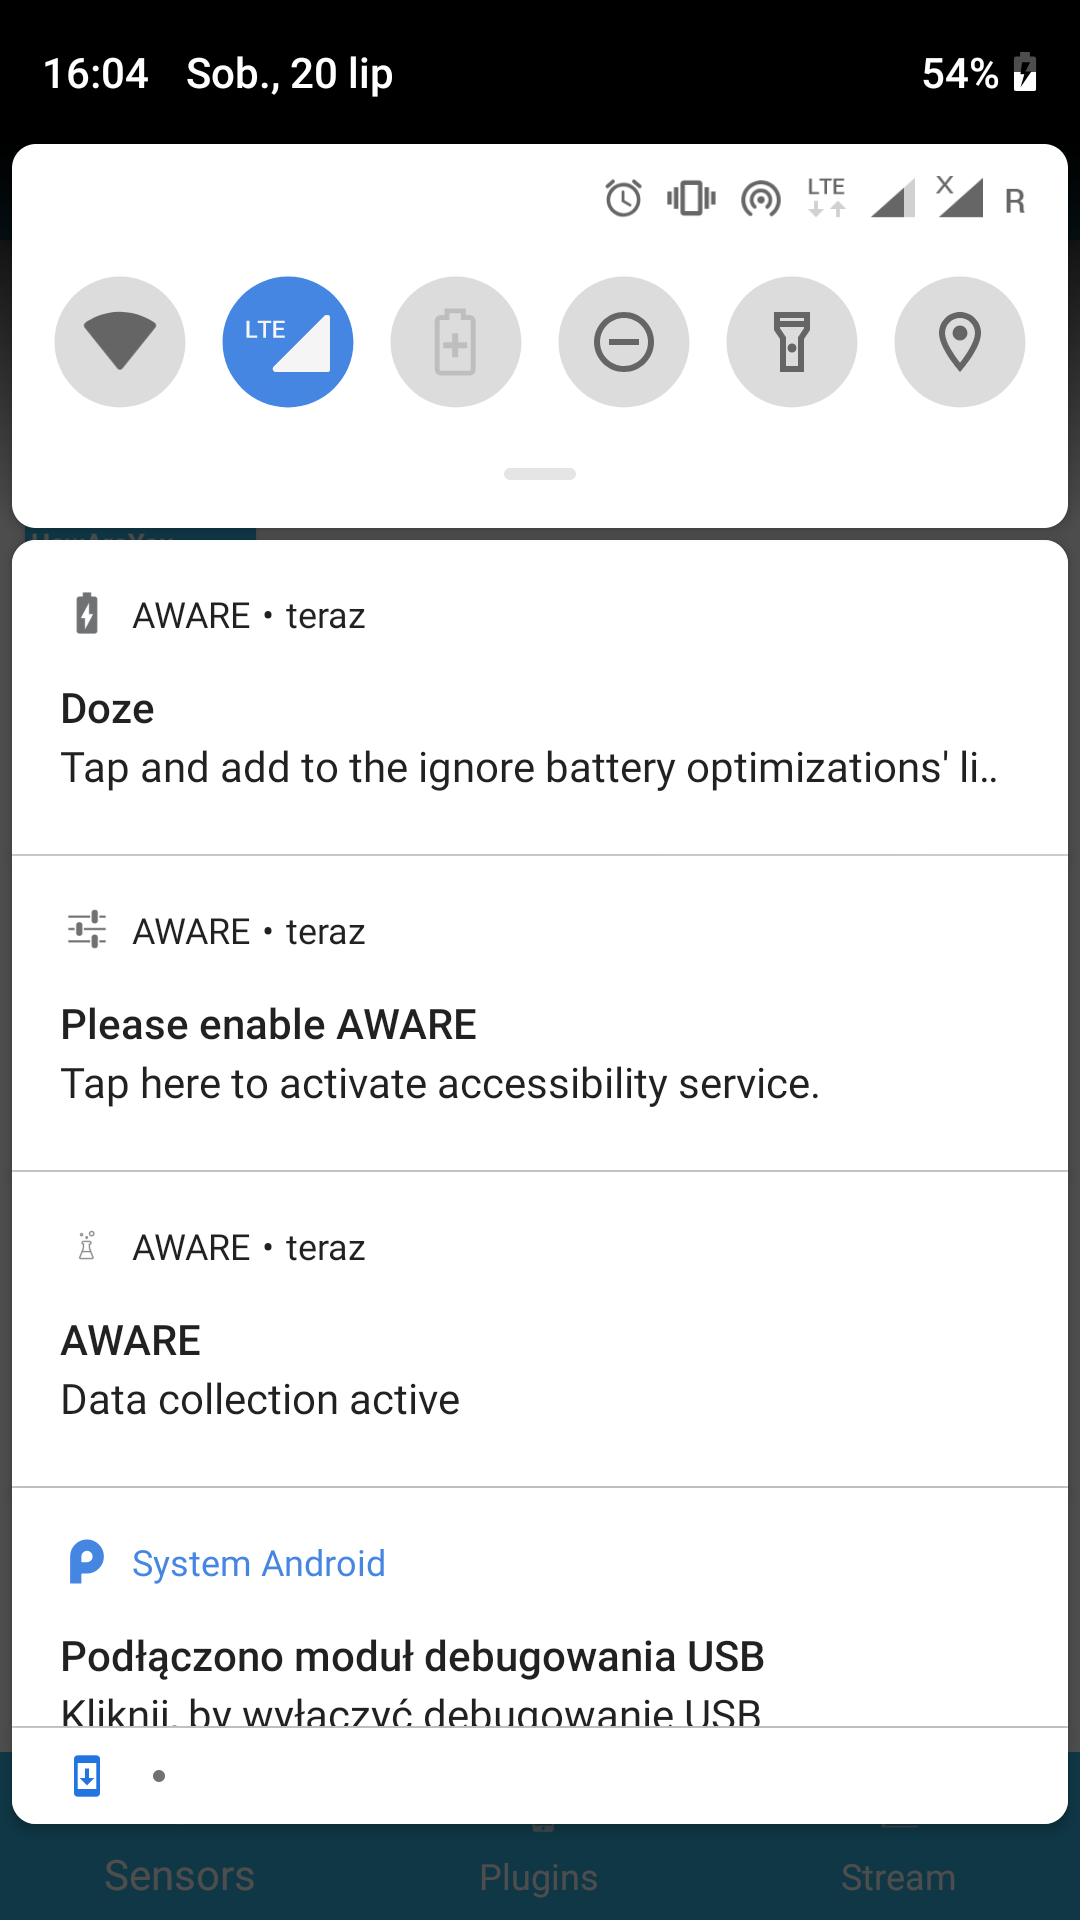
\includegraphics[scale=0.14]{dodatekA/3_6.png}
			\subcaption{\label{subfigure_b}}
		\end{subfigure}
		\caption{ Kroki 5 i 6: Widok zapytania użytkownika o zgodę (a) oraz powiadomienie \textit{Please enable AWARE} (b).}
	\end{figure}
	\clearpage 
	
	\item Kliknij na aplikację \textit{AWARE} i przyznaj uprawnienia klikając \textit{Użyj usługi}. Następnie kliknij na plugin \textit{HowAreYou} i przyznaj uprawnienia klikając \textit{Użyj usługi}.
	
	\item Jeżeli pojawi się powiadomienie \textit{Tap and add to the ignore battery optimizations' list}, kliknij na obszar powiadomienia.
	
	\begin{figure}[H]
		\centering
		\begin{subfigure}{0.35\textwidth}
			\centering
			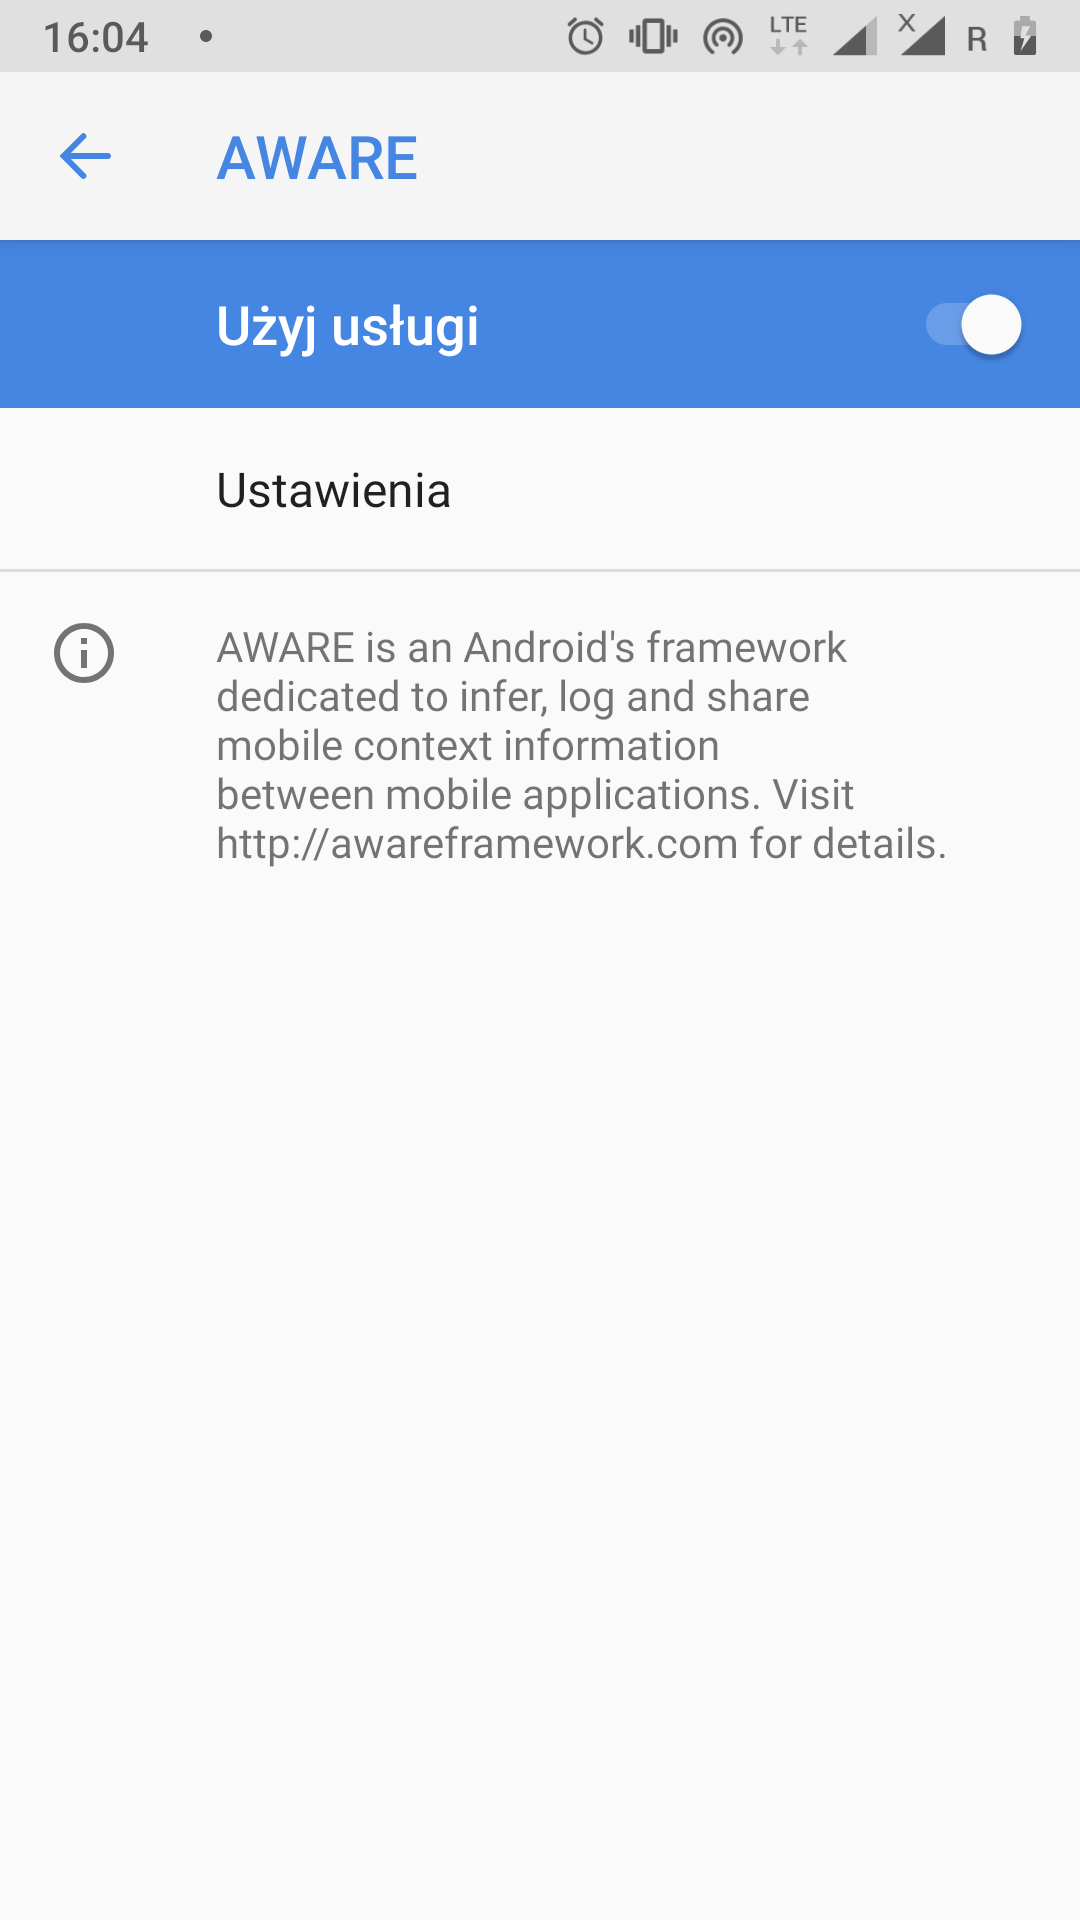
\includegraphics[scale=0.14]{dodatekA/3_7.png}
			\subcaption{\label{subfigure_a}}
		\end{subfigure}
		\begin{subfigure}{0.35\textwidth}
			\centering
			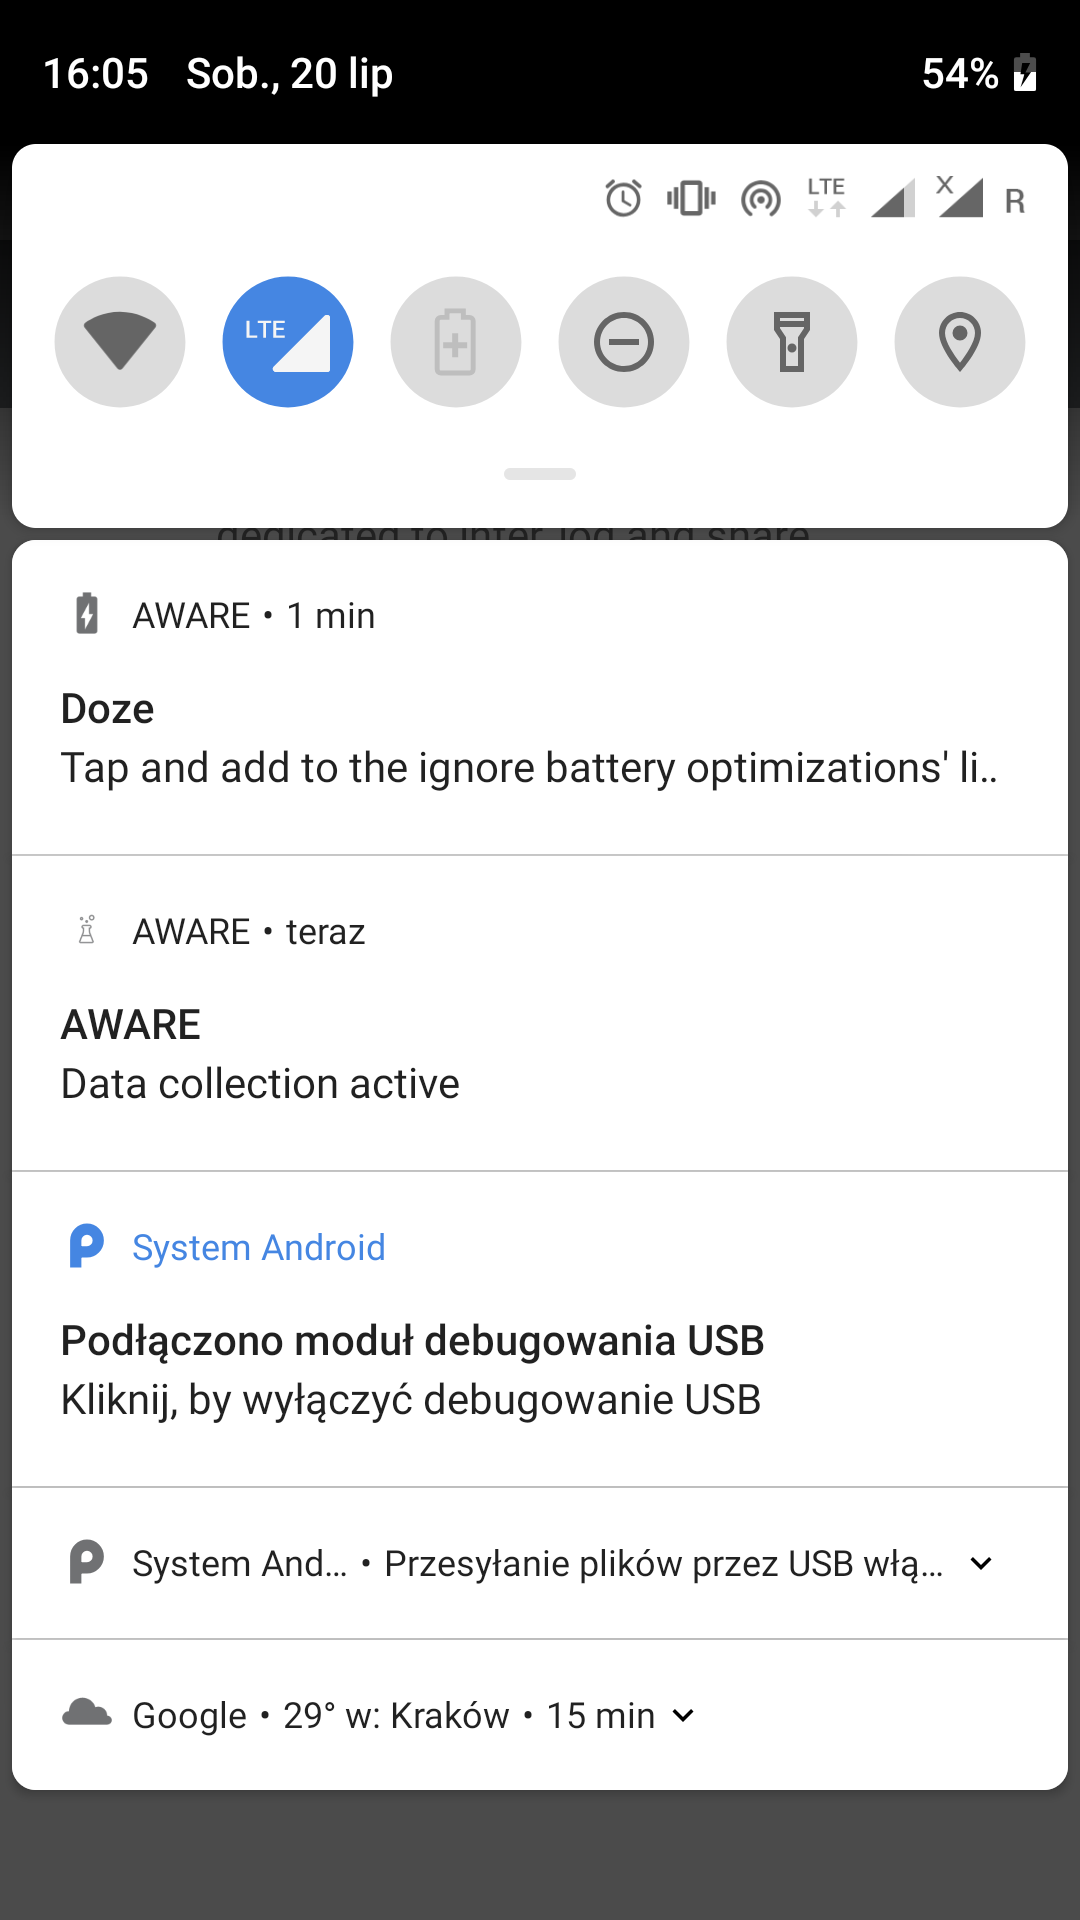
\includegraphics[scale=0.14]{dodatekA/3_8.png}
			\subcaption{\label{subfigure_b}}
		\end{subfigure}
		\caption{ Kroki 7 i 8: Widok przyznawania uprawnień \textit{Accessibility Service} (a) oraz powiadomienie \textit{Tap and add to the ignore battery optimizations' list} (b).}
	\end{figure}
	\clearpage 
	
	\item Wybierz \textit{Pokaż wszystkie aplikacje}.
	
	\item Zarówno na aplikacji \textit{AWARE} jak i na pluginie \textit{HowAreYou} wybierz \textit{Nie Optymalizuj}.
	
	\begin{figure}[H]
		\centering
		\begin{subfigure}{0.35\textwidth}
			\centering
			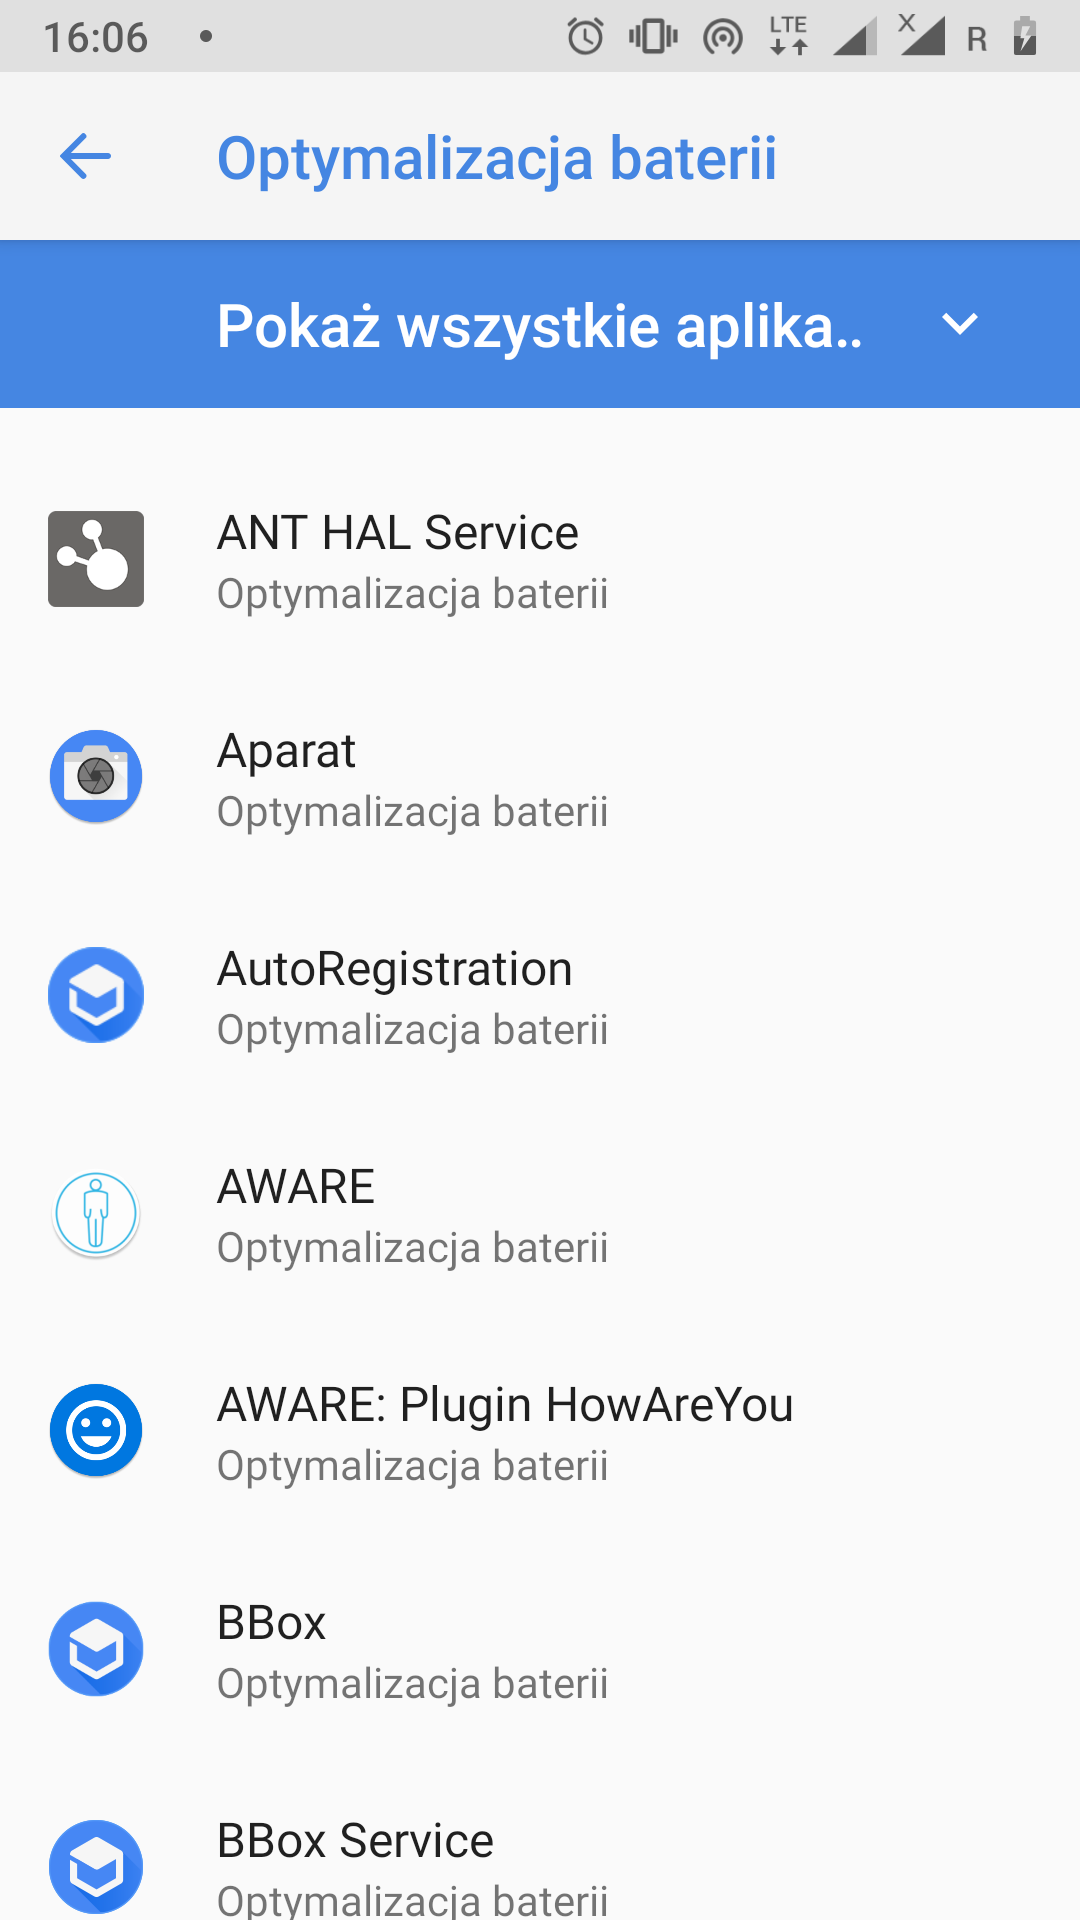
\includegraphics[scale=0.14]{dodatekA/3_9.png}
			\subcaption{\label{subfigure_a}}
		\end{subfigure}
		\begin{subfigure}{0.35\textwidth}
			\centering
			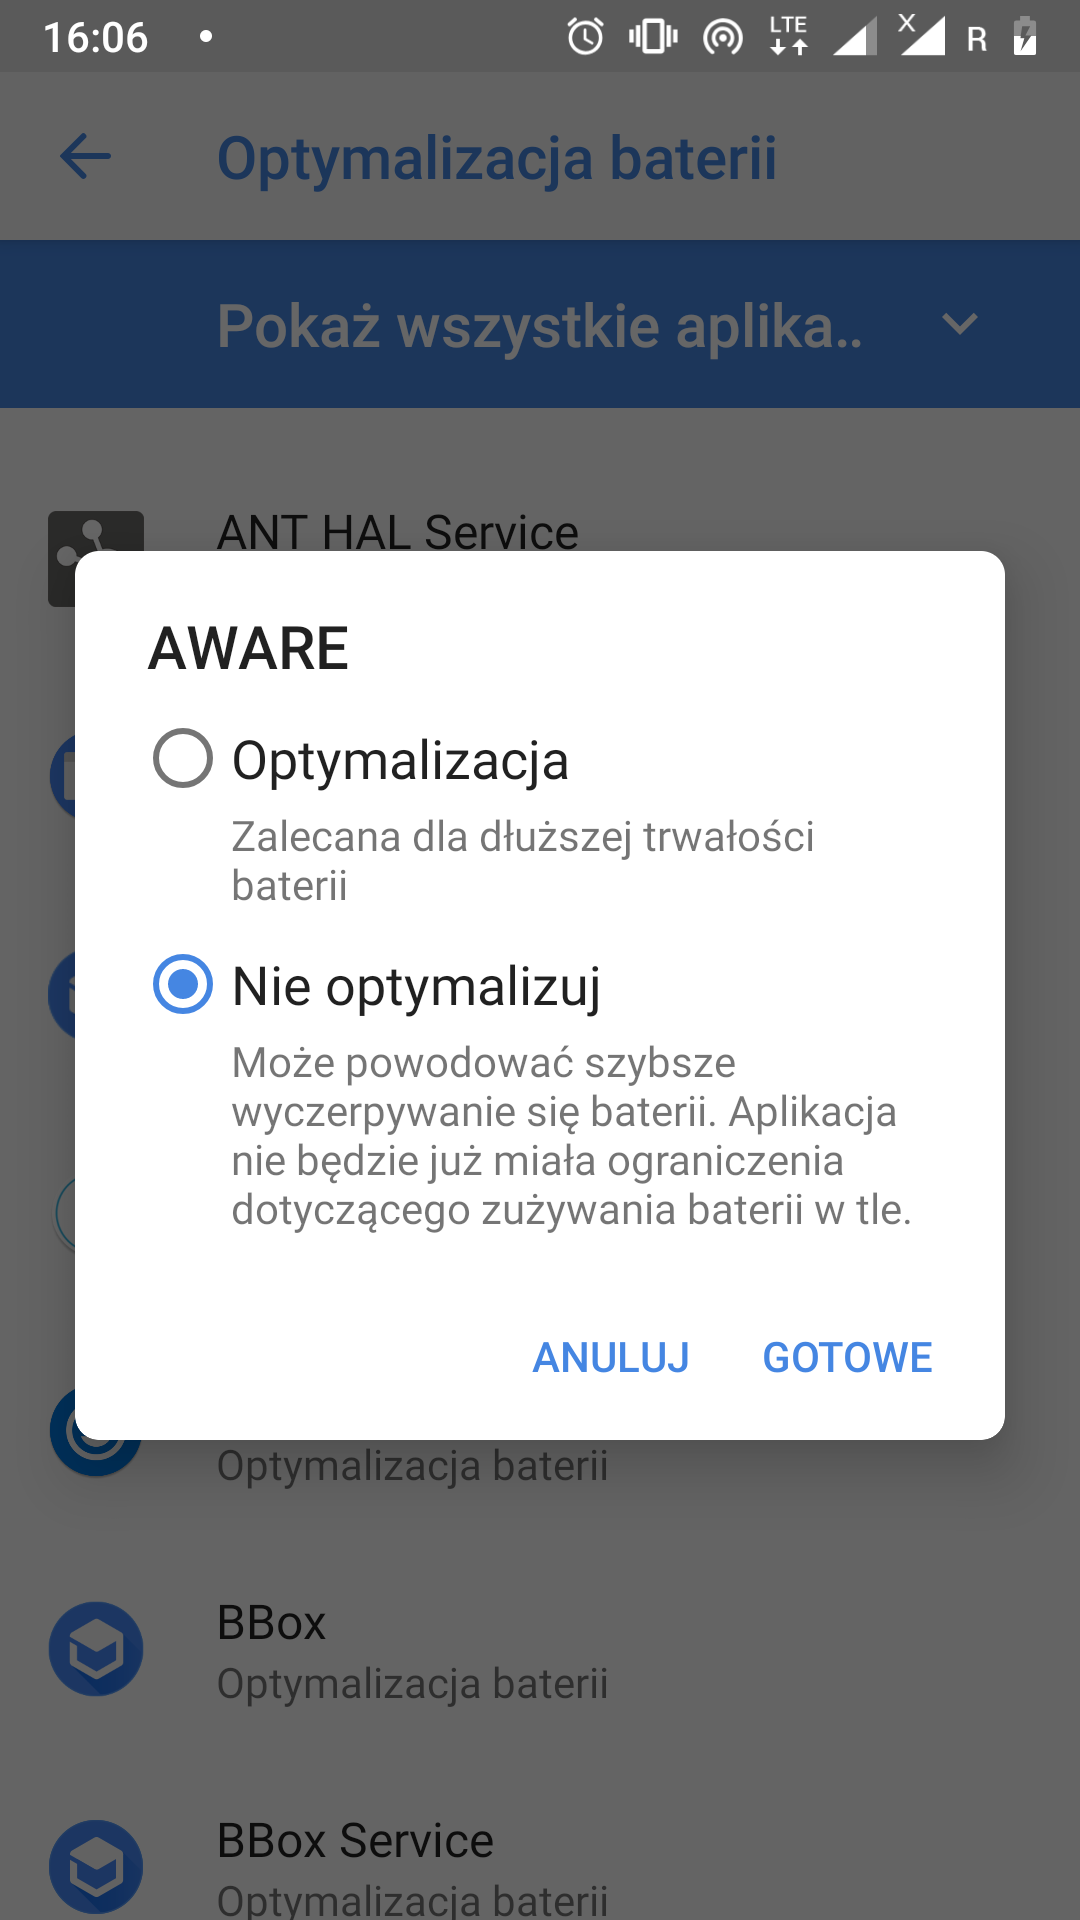
\includegraphics[scale=0.14]{dodatekA/3_10.png}
			\subcaption{\label{subfigure_b}}
		\end{subfigure}
		\caption{ Kroki 9 i 10: Menu ustawień \textit{Optymalizacja Baterii} (a) oraz menu wyboru decyzji (b).}
	\end{figure}
	\clearpage 
 
\end{enumerate}


